
\chapter{Entwurf}
\section{Generelles Abfragen von Daten} \label{data-fetching}
Dieses Abschnitt baut auf das Kapitel \ref{oauth2-strat} auf.
\begin{figure}[!ht]
  \centering
  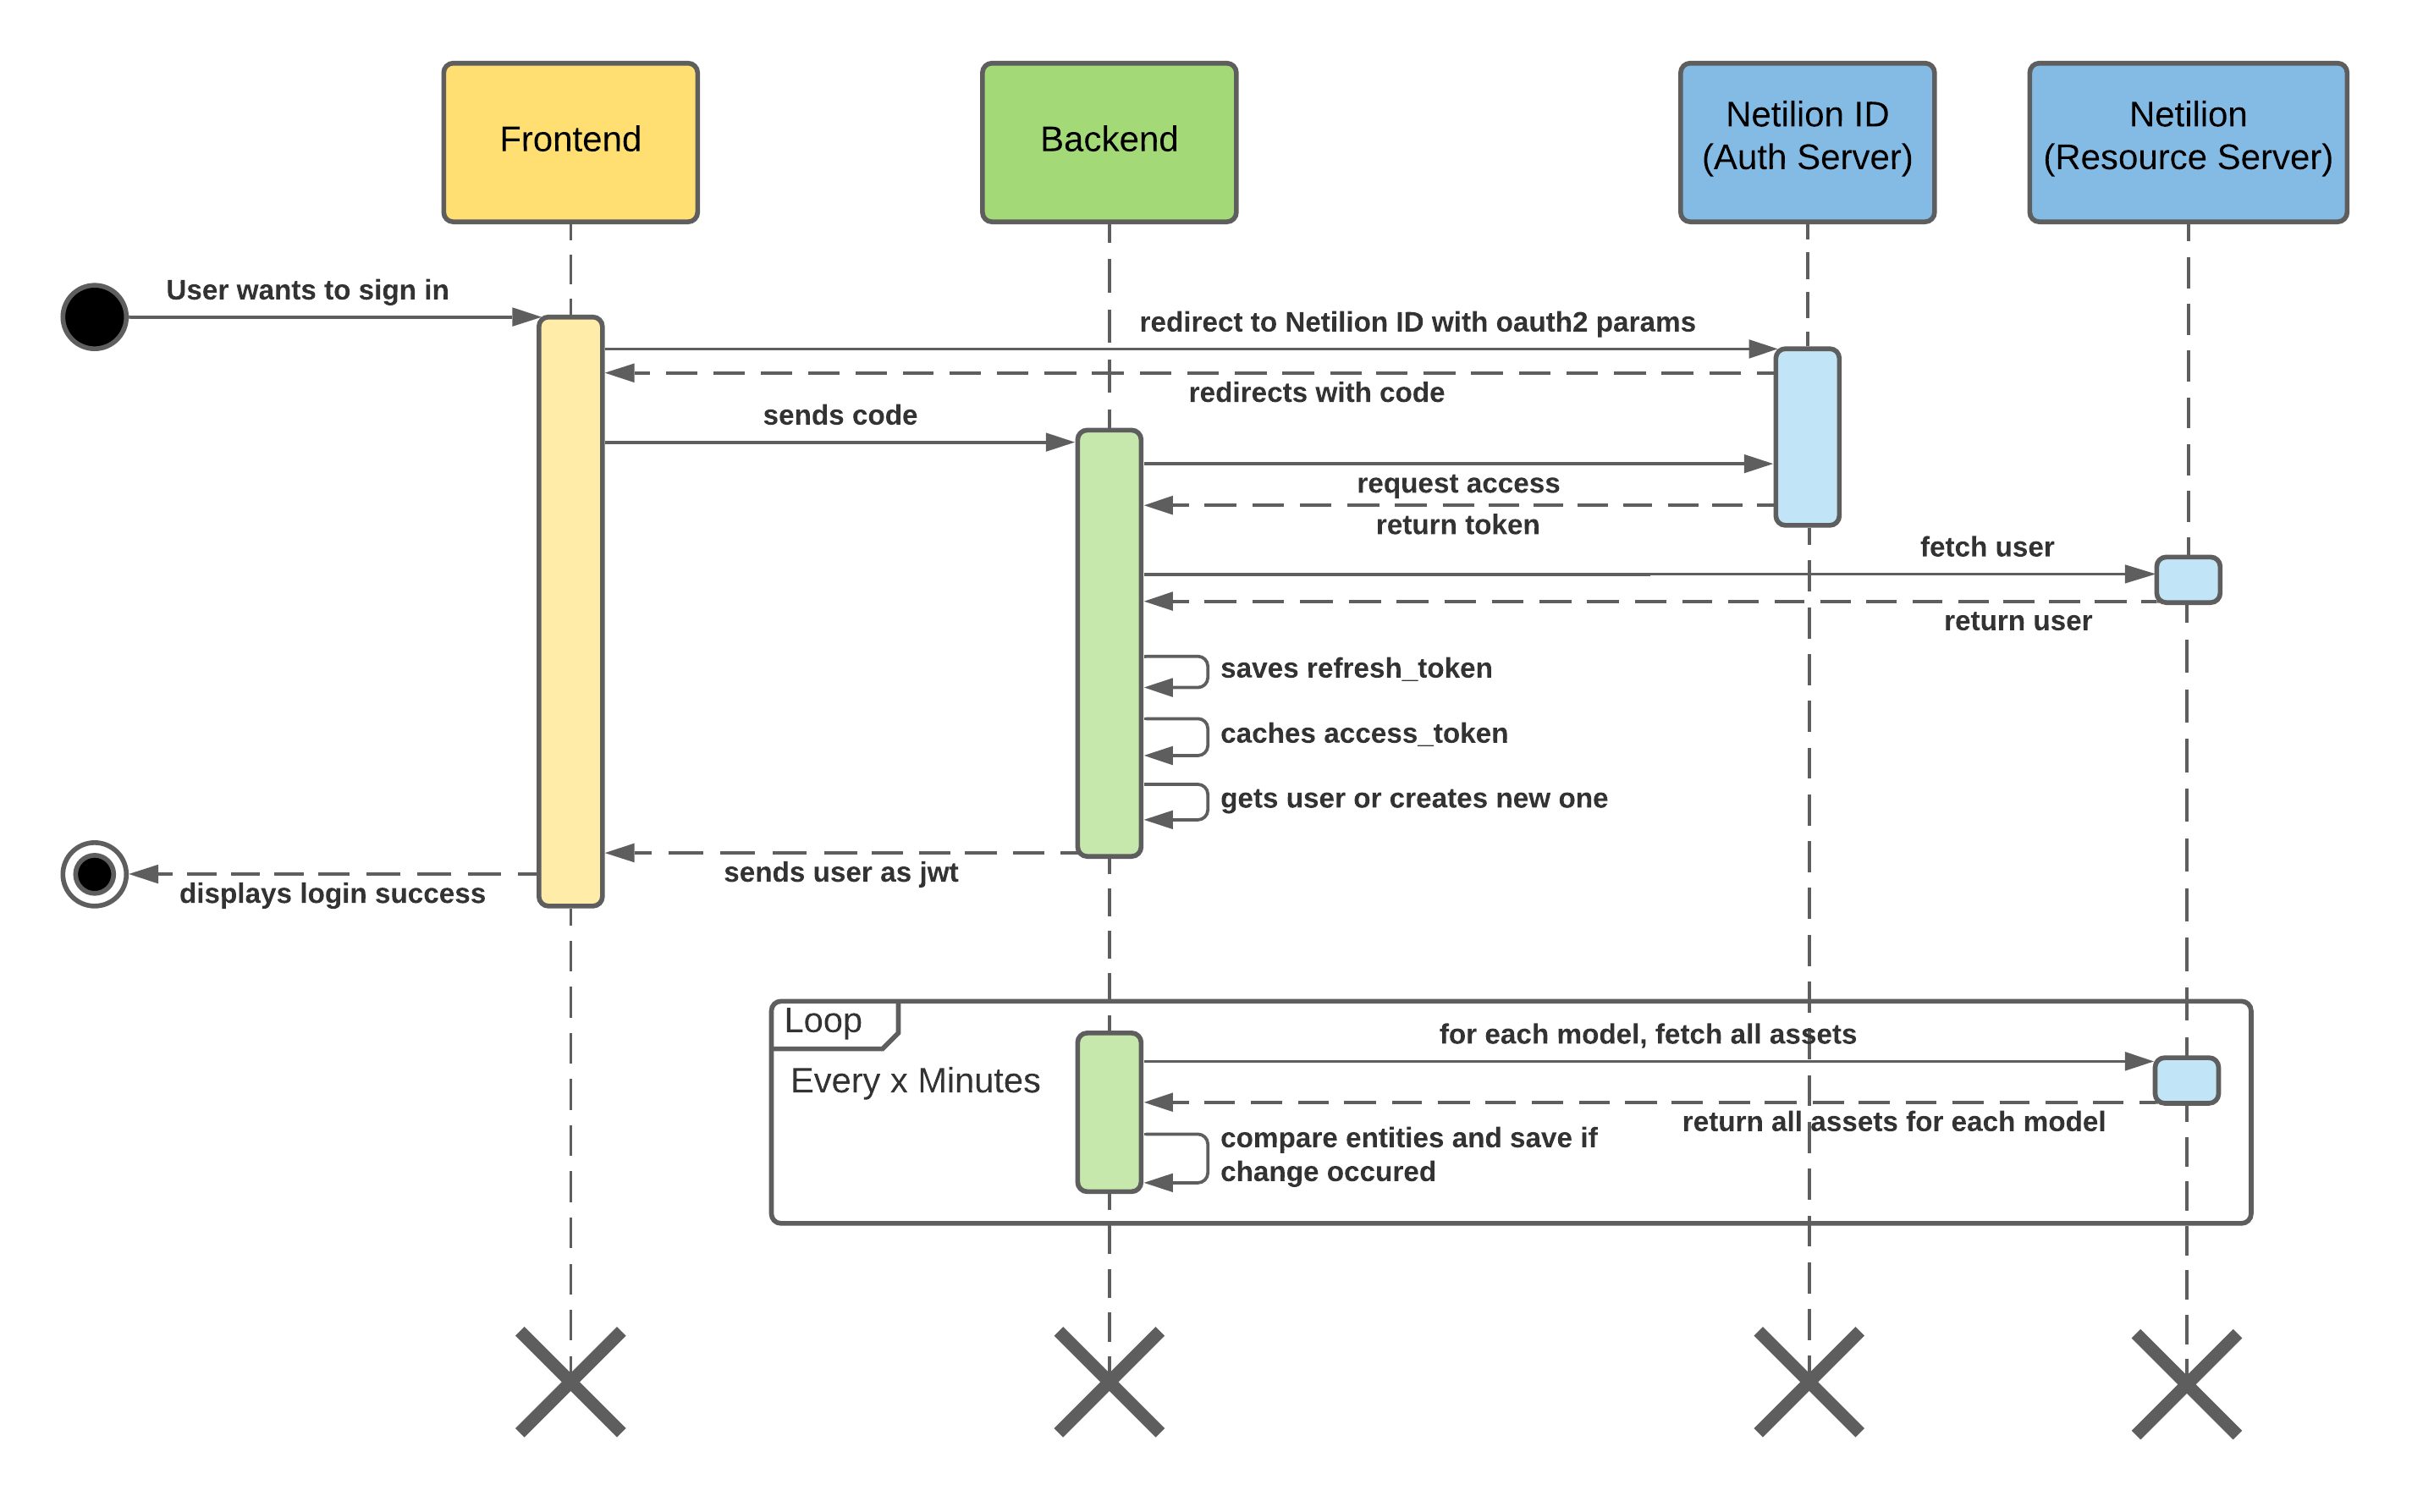
\includegraphics[width=.95\linewidth]{./images/datafetching.png}
  \caption[{Sequenzdiagram, welches das automatische fetching Erklärt}]{Data fetching in Intervallen}
  \label{fig:data-fetching}
\end{figure}
Nachdem sich ein OSE Verantwortlicher das erste mal eingeloggt hat, wird der \code{access\_token} in Redis gecached und der \code{refresh\_token} in der Datenbank gespeichert. Die Funktion soll entweder den gecachten Token nehmen und direkt zurückgeben oder mit dem \code{refresh\_token} einen neuen Anfordern, welcher wiederum gecached und zurückgegeben werden soll. Damit ist es dann möglich, dass das Backend selbst die Daten auffrischen kann. Dafür werde ich das Task-Scheduling\cite{a2021_documentation} feature von Nestjs verwenden. Damit ist es möglich eine Funktion wiederholt laufen zu lassen.
\newline
Bevor ich allerdings das ganze automatisieren kann, brauche ich eine Helferfunktion. Denn jede Anfrage an Netilion braucht einen validen \code{access\_token} und er muss auch dem Netilion Benutzer gehören, unter welchem die Messgeräte registriert sind. Mit dieser Function wird es möglich sein das ganze zu vollautomatisieren. Wenn nun ein Benutzer des OSE-Dashboards sich die Daten nun ansehen möchte, kann er dies machen, ohne den Login des jeweiligen OSE Verantwortlichen wissen zu müssen.
\pagebreak
\section{Zugriffskontrolle}
\subsection{OSE Verantwortlicher}
\begin{figure}[H]
  \centering
  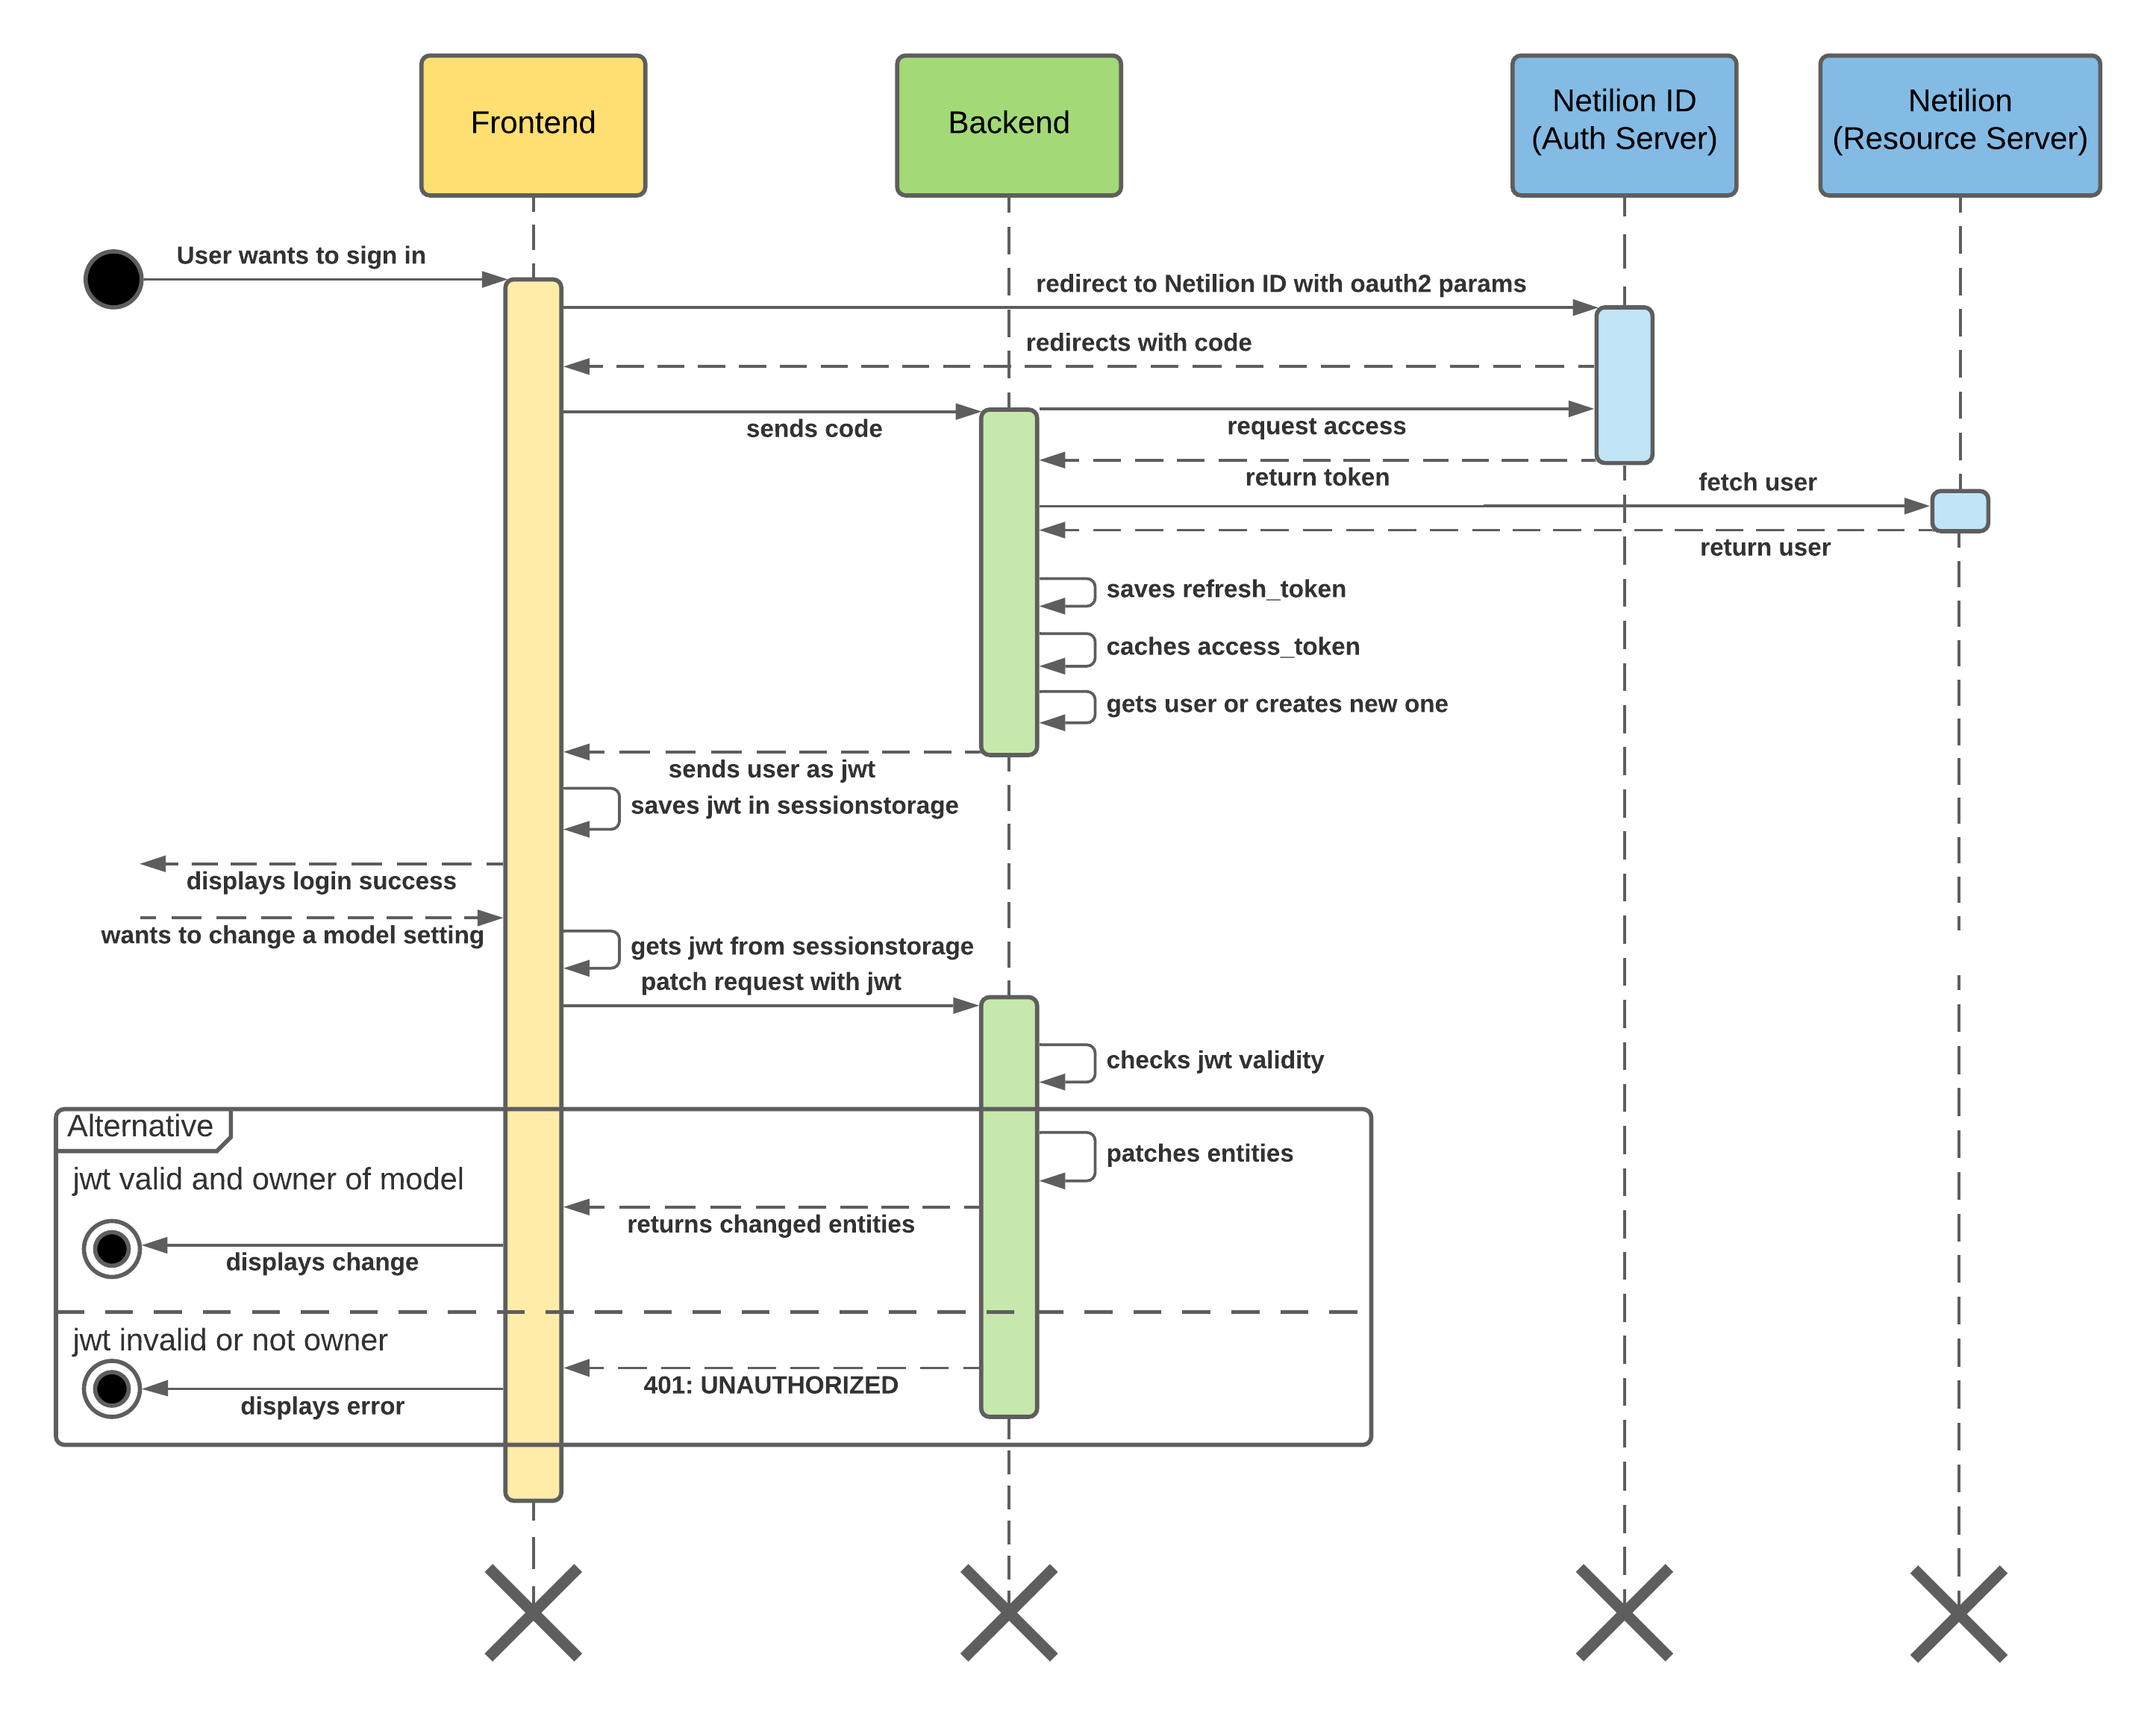
\includegraphics[width=.95\linewidth]{./images/zugriffskontrolle.png}
  \caption[{Sequenzdiagram, welches die Zugriffskontrolle für den OSE Verantwortlichen beschreibt}]{Zugriffskontrolle OSE Verantwortlicher}
  \label{fig:zugriffskontrolle}
\end{figure}
Ein OSE Verantwortlicher soll das Konfigurationsmenü seines Modells öffnen können. Verantwortlicher anderer Modelle oder normale User sollen dies nicht können.
Das ganze sollte folgenderweise gelöst werden:
\newline
Das Frontend erhält nach dem erfolgreichen Login einen JWT. Dieser wird zuerst benötigt, um den Link zum Konfigurationsmenü überhaupt erst im Frontend anzuzeigen. Ausserdem wird er als Authentifizierungsmethode zum Backend verwendet. Der REST Endpoint vom Backend wird durch eine Nestjs Guard\cite{nest_guards} geschützt. Daraufhin wird direkt geprüft werden, ob das Modell auch wirklich dem User gehört. Sollte dies nicht der Fall sein, wird die Anfrage als unauthorized zurückgeschickt.
\subsection{OSE-Dashboard Nutzer}
\begin{figure}[H]
  \centering
  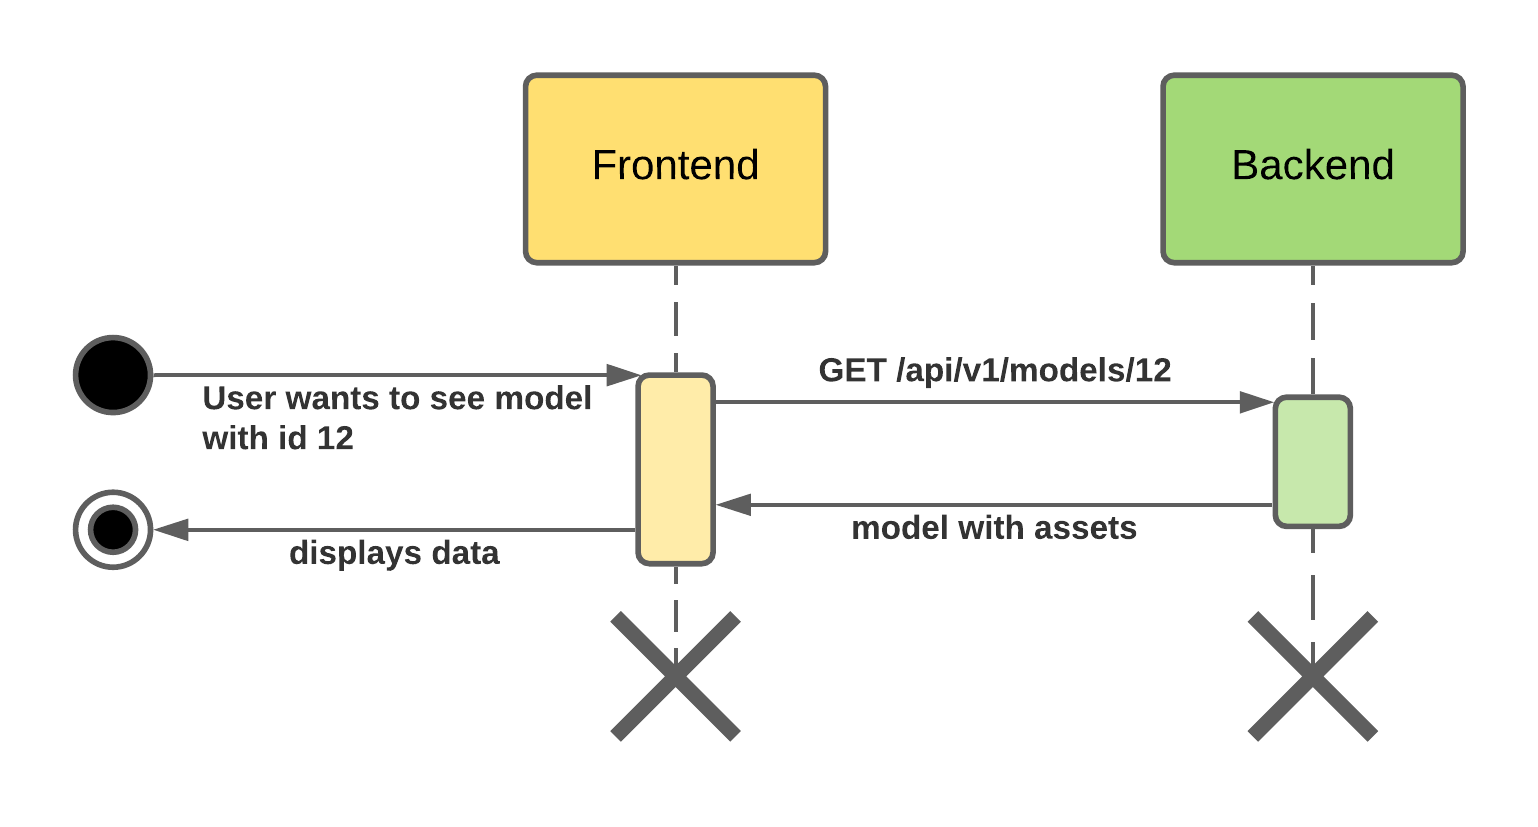
\includegraphics[width=.6\linewidth]{./images/zugriffskontrolle2.png}
  \caption[{Sequenzdiagram, welches die Zugriffskontrolle für den OSE-Dashboard Nutzer beschreibt}]{Zugriffskontrolle OSE-Dashboard Nutzer}
  \label{fig:zugriffskontrolle2}
\end{figure}
Der OSE-Dashboard möchte sich alle OSE-Modelle ansehen können, ohne sich dabei einloggen zu müssen.
Das ganze sollte folgenderweise gelöst werden:
\newline
Wie in Kapitel \ref{data-fetching} angesprochen, sind die aktuellen Daten im Backend verfügbar. So ist es also gar nicht nötig Netilion direkt anzufragen. Das Backend soll stattdessen die Daten mit einem public Endpoint verfügbar machen. Auf diesem Weg umgehen wir auch die maximale Anfragen an Netilion, welche in Kapitel \ref{arch-backend} beschrieben wurde.
\newline
So kann das Frontend beliebig oft die Daten abfragen, ohne das sich ein User einloggen muss oder das wir die Grenze der Connect Subscription übertreten.
\section{Softwareschnittstellen}
Die zu erweiterbare Webapplikation ist in mehrere logische Schichten unterteilt. Jede Schicht ist für einen konkreten Teil der kompletten Lösung verandwortlich. Eine vereinfachte Darstellung der Lösung ist bereits in der Abbildung \ref{fig:systemarchitektur} dargestellt. Folgend sind alle Schichten und deren Zuständigkeit zusammengefasst:
\begin{table}[H]
  \begin{tabularx}{\textwidth}{l X}\hline \\
  \textbf{Schicht} & \textbf{Zuständigkeit}  \\ \\\hline \\
  OSE & Daten der Messgeräte in der Anlage werden von einem Edge Device gesammelts und an Netilion gesendet \\
  Netilion & IIoT-Service von Endress+Hauser \\
  Backend & Backend des OSE Dashboards \\
  HERE Developer API & API Eines Drittanbieters. Wird verwendet für das Abfragen von Koordinaten oder Addressen und für die Darstellung der Karte. \\
  Frontend & Frontend des OSE Dashboards \\
  \\\hline
  \end{tabularx}
\end{table}
\subsection{Schnittstellen im OSE}
Wie und welche Daten das OSE Modell an Netilion schickt ist für diese Arbeit nicht relevant und wird daher nicht dokumentiert. Allerdings ist es wichtig zu wissen, dass die Daten gesammelt und in Intervallen an Netilion gesendet werden.
\subsection{Netilion}
Folgend sind die verwendeten Schnittstellen von Netilion aufgelisted. Von den angeforderten Entitäten werden nur die verwendeten Attribute vermerkt und beschrieben. Um zusätzliche Informationen über die Entitäten zu erhalten, sollten die offizielle \href{https://api.iiot.endress.com/doc/v1/}{Netilion API Dokumentation} aufgesucht werden.
\subsubsection{API Routes}
\begin{table}[H]
  \begin{tabularx}{\textwidth}{l X X}\hline \\
  \textbf{Anfrage} & \textbf{Pfad} & \textbf{Antwort}  \\ \\\hline \\
  HTTP:GET & \code{/users/current} & NetilionUser \\
  HTTP:GET & \code{/assets} & Array of Asset \\
  \\\hline
  \end{tabularx}
\end{table}
\subsubsection{NetilionUser}
\begin{table}[H]
  \begin{tabularx}{\textwidth}{l l X}\hline \\
  \textbf{Attribut} & \textbf{Datentyp} & \textbf{Beschreibung}  \\ \\\hline \\
  id & number & Primary Key \\
  email & string & Email mit der sich der Nutzer auf Netilion registriert hat \\
  \\\hline
  \end{tabularx}
\end{table}
\subsubsection{Asset}
\begin{table}[H]
  \begin{tabularx}{\textwidth}{l l X}\hline \\
  \textbf{Attribut} & \textbf{Datentyp} & \textbf{Beschreibung}  \\ \\\hline \\
  id & number & Primary Key \\
  serial\_number & string & Seriennummer des Messgerätes \\
  description & string & Beschreibung des Messgerätes \\
  production\_date & string & Produktionsdatum des Messgerätes \\
  last\_seen\_at & string & Wann sich das Messgerät zuletz bei Netilion gemeldet hat \\
  product & number & Foreign Key\\
  status & number & Foreign Key \\
  instrumentations & number & Foreign Key \\
  \\\hline
  \end{tabularx}
\end{table}
\subsubsection{Status}
Der Health-Status des Messgerätes. Zeigt zum Beispiel an, ob das Gerät gewartet werden muss.
\begin{table}[H]
  \begin{tabularx}{\textwidth}{l l X}\hline \\
    \textbf{Attribut} & \textbf{Datentyp} & \textbf{Beschreibung}  \\ \\\hline \\
    id & number & Primary Key \\
    code & string & Standartisierter Status Code \\
    description & string & Beschreibung des Status \\
    name & string & Name des standartisierten Status Codes \\
    \\\hline
  \end{tabularx}
\end{table}
\subsubsection{Instrumentations}
Instrumentations ist der interne Begriff für die Messstelle, an der sich das Messgerät befindet. Wird auch Tag genannt.
\begin{table}[H]
  \begin{tabularx}{\textwidth}{l l X}\hline \\
    \textbf{Attribut} & \textbf{Datentyp} & \textbf{Beschreibung}  \\ \\\hline \\
    id & number & Primary Key \\
    tag & string & Bezeichnung der Messstelle \\
    description & string & Beschreibung der Messstelle \\
    criticality & string & Kritikalität der Messstelle \\
    accessibility & string & Erreichbarkeit der Messstelle \\
    \\\hline
  \end{tabularx}
\end{table}
\subsubsection{Product}
Ein Product ist ein Typ von Messgerät. Product bildet dabei das allgemeine Produkt ab, während dem Asset ein Zwilling eines hergestellten Messgerätes vom Typ Product ist.
\begin{table}[H]
  \begin{tabularx}{\textwidth}{l l X}\hline \\
  \textbf{Attribut} & \textbf{Datentyp} & \textbf{Beschreibung}  \\ \\\hline \\
  id & number & Primary Key \\
  product\_code & string & Code des Produktes \\
  name & string & Name des Produktes \\
  description & string & Beschreibung des Produktes \\
  manufacturer & number & Foreign Key \\
  \\\hline
  \end{tabularx}
\end{table}
\subsubsection{Manufacturer}
Der Manufacturer ist der Hersteller eines Messgerätes.
\begin{table}[H]
  \begin{tabularx}{\textwidth}{l l X}\hline \\
  \textbf{Attribut} & \textbf{Datentyp} & \textbf{Beschreibung}  \\ \\\hline \\
  id & number & Primary Key \\
  name& string & Name des Herstellers \\
  \\\hline
  \end{tabularx}
\end{table}
\pagebreak
\subsection{Backend}
Folgend sind die verwendeten Schnittstellen von \code{ose-dashboard-bcknd} aufgelisted.
\subsubsection{API Routes}
\begin{table}[H]
  \begin{tabularx}{\textwidth}{l X X}\hline \\
  \textbf{Anfrage} & \textbf{Pfad} & \textbf{Antwort}  \\ \\\hline \\
  \textbf{Models} & & \\
  HTTP:POST & \code{/models/:modelId/assets/:assetId} & Void \\
  HTTP:POST & \code{/models/:id/autolink} & Void \\
  HTTP:POST & \code{/register} & Model \\
  HTTP:GET & \code{/models} & Array of Models \\
  HTTP:GET & \code{/models/:id} & Model \\
  HTTP:GET & \code{/models/:id/location} & Location \\
  HTTP:GET & \code{/models/:id/assets} & Array of Asset \\
  HTTP:PUT & \code{/models/:id/location} & Location \\
  HTTP:PATCH & \code{/models/:id} & Model \\
  \textbf{Assets} & & \\
  HTTP:GET & \code{/assets} & Array of Assets \\
  HTTP:GET & \code{/assets/:id} & Asset \\
  \textbf{Users} & & \\
  HTTP:GET & \code{/users/current} & Array of Assets \\
  HTTP:GET & \code{/users/:id/model} & Model \\
  HTTP:PATCH & \code{/users/:id/finished-setup} & Void \\
  \textbf{Location} & & \\
  HTTP:GET & \code{/mapview} & \code{image/jpeg; charset=UTF-8} \\
  HTTP:GET & \code{/geolocation} & Array of Locations \\
  \textbf{Authentication} & & \\
  HTTP:POST & \code{/auth/login} & Void \\
  \\\hline
  \end{tabularx}
\end{table}
\subsubsection{Model}
Digitale Abbildung eines OSE Modelles
\begin{table}[H]
  \begin{tabularx}{\textwidth}{l l X}\hline \\
  \textbf{Attribut} & \textbf{Datentyp} & \textbf{Beschreibung}  \\ \\\hline \\
  id & number & Primary Key \\
  name & string & Name des Modelles \\
  description & string & Beschreibung des Modelles \\
  location & string & Id der Addresse des Modelles \\
  owner & number & Foreign Key \\
  assets & number & Foreign Key \\
  \\\hline
  \end{tabularx}
\end{table}
\subsection{HERE Developer API}
Diese API ermöglicht die Ortung der Modelle in diesem Projekt. Sie ermöglicht das Abfragen von Addressen und das rendern von Satelitenkarten. Um diese Daten abzufragen, wird allerdings ein ApiKey benötigt. Diese API soll nicht im Frontend abgefragt werden, da ansonsten dieser Key abgegriffen werden kann. Die beiden folgend beschriebenen API-Routen sollen daher über das Backend proxied werden, wo der APIKey im nachhinein der Anfrage beigefügt wird.
\subsubsection{API Routes}
\begin{table}[H]
  \begin{tabularx}{\textwidth}{l X X}\hline \\
  \textbf{Anfrage} & \textbf{Pfad} & \textbf{Antwort}  \\ \\\hline \\
  HTTP:GET & \code{/v1/geocode} & Array of Locations \\
  HTTP:GET & \code{/mia/1.6/mapview} & \code{image/jpeg; charset=UTF-8} \\
  \\\hline
  \end{tabularx}
\end{table}
\subsubsection{Location}
\begin{table}[H]
  \begin{tabularx}{\textwidth}{l l X}\hline \\
  \textbf{Attribut} & \textbf{Datentyp} & \textbf{Beschreibung}  \\ \\\hline \\
  id & string & Eindeutige Identifikationsnummer \\
  title & string & Ausgeschriebene Adresse \\
  position & object & Objekt, welches den Längengrad und Breitengrad enthält \\
  \\\hline
  \end{tabularx}
\end{table}
\subsection{Frontend}
Das Frontend ist mit Nextjs gemacht und baut auf React auf. Es konsumiert Daten des Backends und stellt diese passend dar. Vorhandene Schnittstellen dienen nicht für andere Software, sondern für die Interaktion mit Kunden.
\begin{table}[H]
  \begin{tabularx}{\textwidth}{l l X}\hline \\
  \textbf{Geschützt?} & \textbf{Pfad} & \textbf{Funktionalität}  \\ \\\hline \\
  Nein & \code{/} & Zeigt die Startseite an \\
  Nein & \code{/models/:id} & Zeigt selektierte 3D Model an \\
  Nein & \code{/register} & Zeigt selektierte 3D Model an \\
  Nein & \code{/register/error} & Zeigt Fehlermeldung an und leited Benutzer nach 15 Sekunden weiter an die Startseite \\
  Nein & \code{/register/unauthorized} & Zeigt Fehlermeldung an und leited Benutzer nach 15 Sekunden weiter an die Startseite \\
  Ja & \code{/settings} & Leitet weiter auf \code{/settings/model} \\
  Ja & \code{/settings/model} & Zeigt Einstellungsmenü des Modelles an \\
  Ja & \code{/settings/location} & Zeigt Einstellungsmenü des Standortes an \\
  Ja & \code{/settings/assets} & Zeigt Einstellungsmenü der Verlinkungen an \\
  \\\hline
  \end{tabularx}
\end{table}
\section{Mockups}
Mockups dienen zur Planung der Darstellung des Frontends. Es ist viel sinnvoller das Layout und den Inhalt der Website im Vorfeld zu skizzieren und damit herumzuspielen, als während dem Implementieren. Weiss man während der Implementierungsphase noch nicht wie das Produkt grob aussehen sollte verschwendet man meist wertvolle Zeit.
\newline
Oft wird vor der Erstellung der Website ein UX-Design erstellt. Dieses gibt grob das Layout und den Inhalt. Ein UI-Design wird angewand wenn das detaillierte Design der Website wichtig ist. Dabei werden die ganzen Komponenten der Website bis ins Detail im Vorfeld designed, sodass dies den Anspruchsgruppen und den Programmieren klar ist.
\newline
Bei dieser Arbeit ist nur die Erarbeitung eines UX-Designs wichtig. Dies wurde soweit erstellt und ist nachfolgend in den Kapiteln dokumentiert.
\pagebreak
\subsection{Index Page} \label{mck:index} 
Momentan ist die Index Page des OSE-Dashboards das Reinacher Modell selbst. Dies soll sich nun ändern. Die rote Linie markiert die initiale Sicht des User. Diese enthält den Titel und eine Beschreibung der Webapplikationen, gefolgt von der Auswahlmöglichkeit der ganzen Modelle. Unter der initialen Sicht ist ein Abschnitt, welcher den User fragt, ob er für ein OSE-Modell zuständig ist. Sollte dies der Fall sein, könne er sich einloggen und so die Daten für das Dashboard zur verfügung stellen.
\begin{figure}[H]
  \centering
  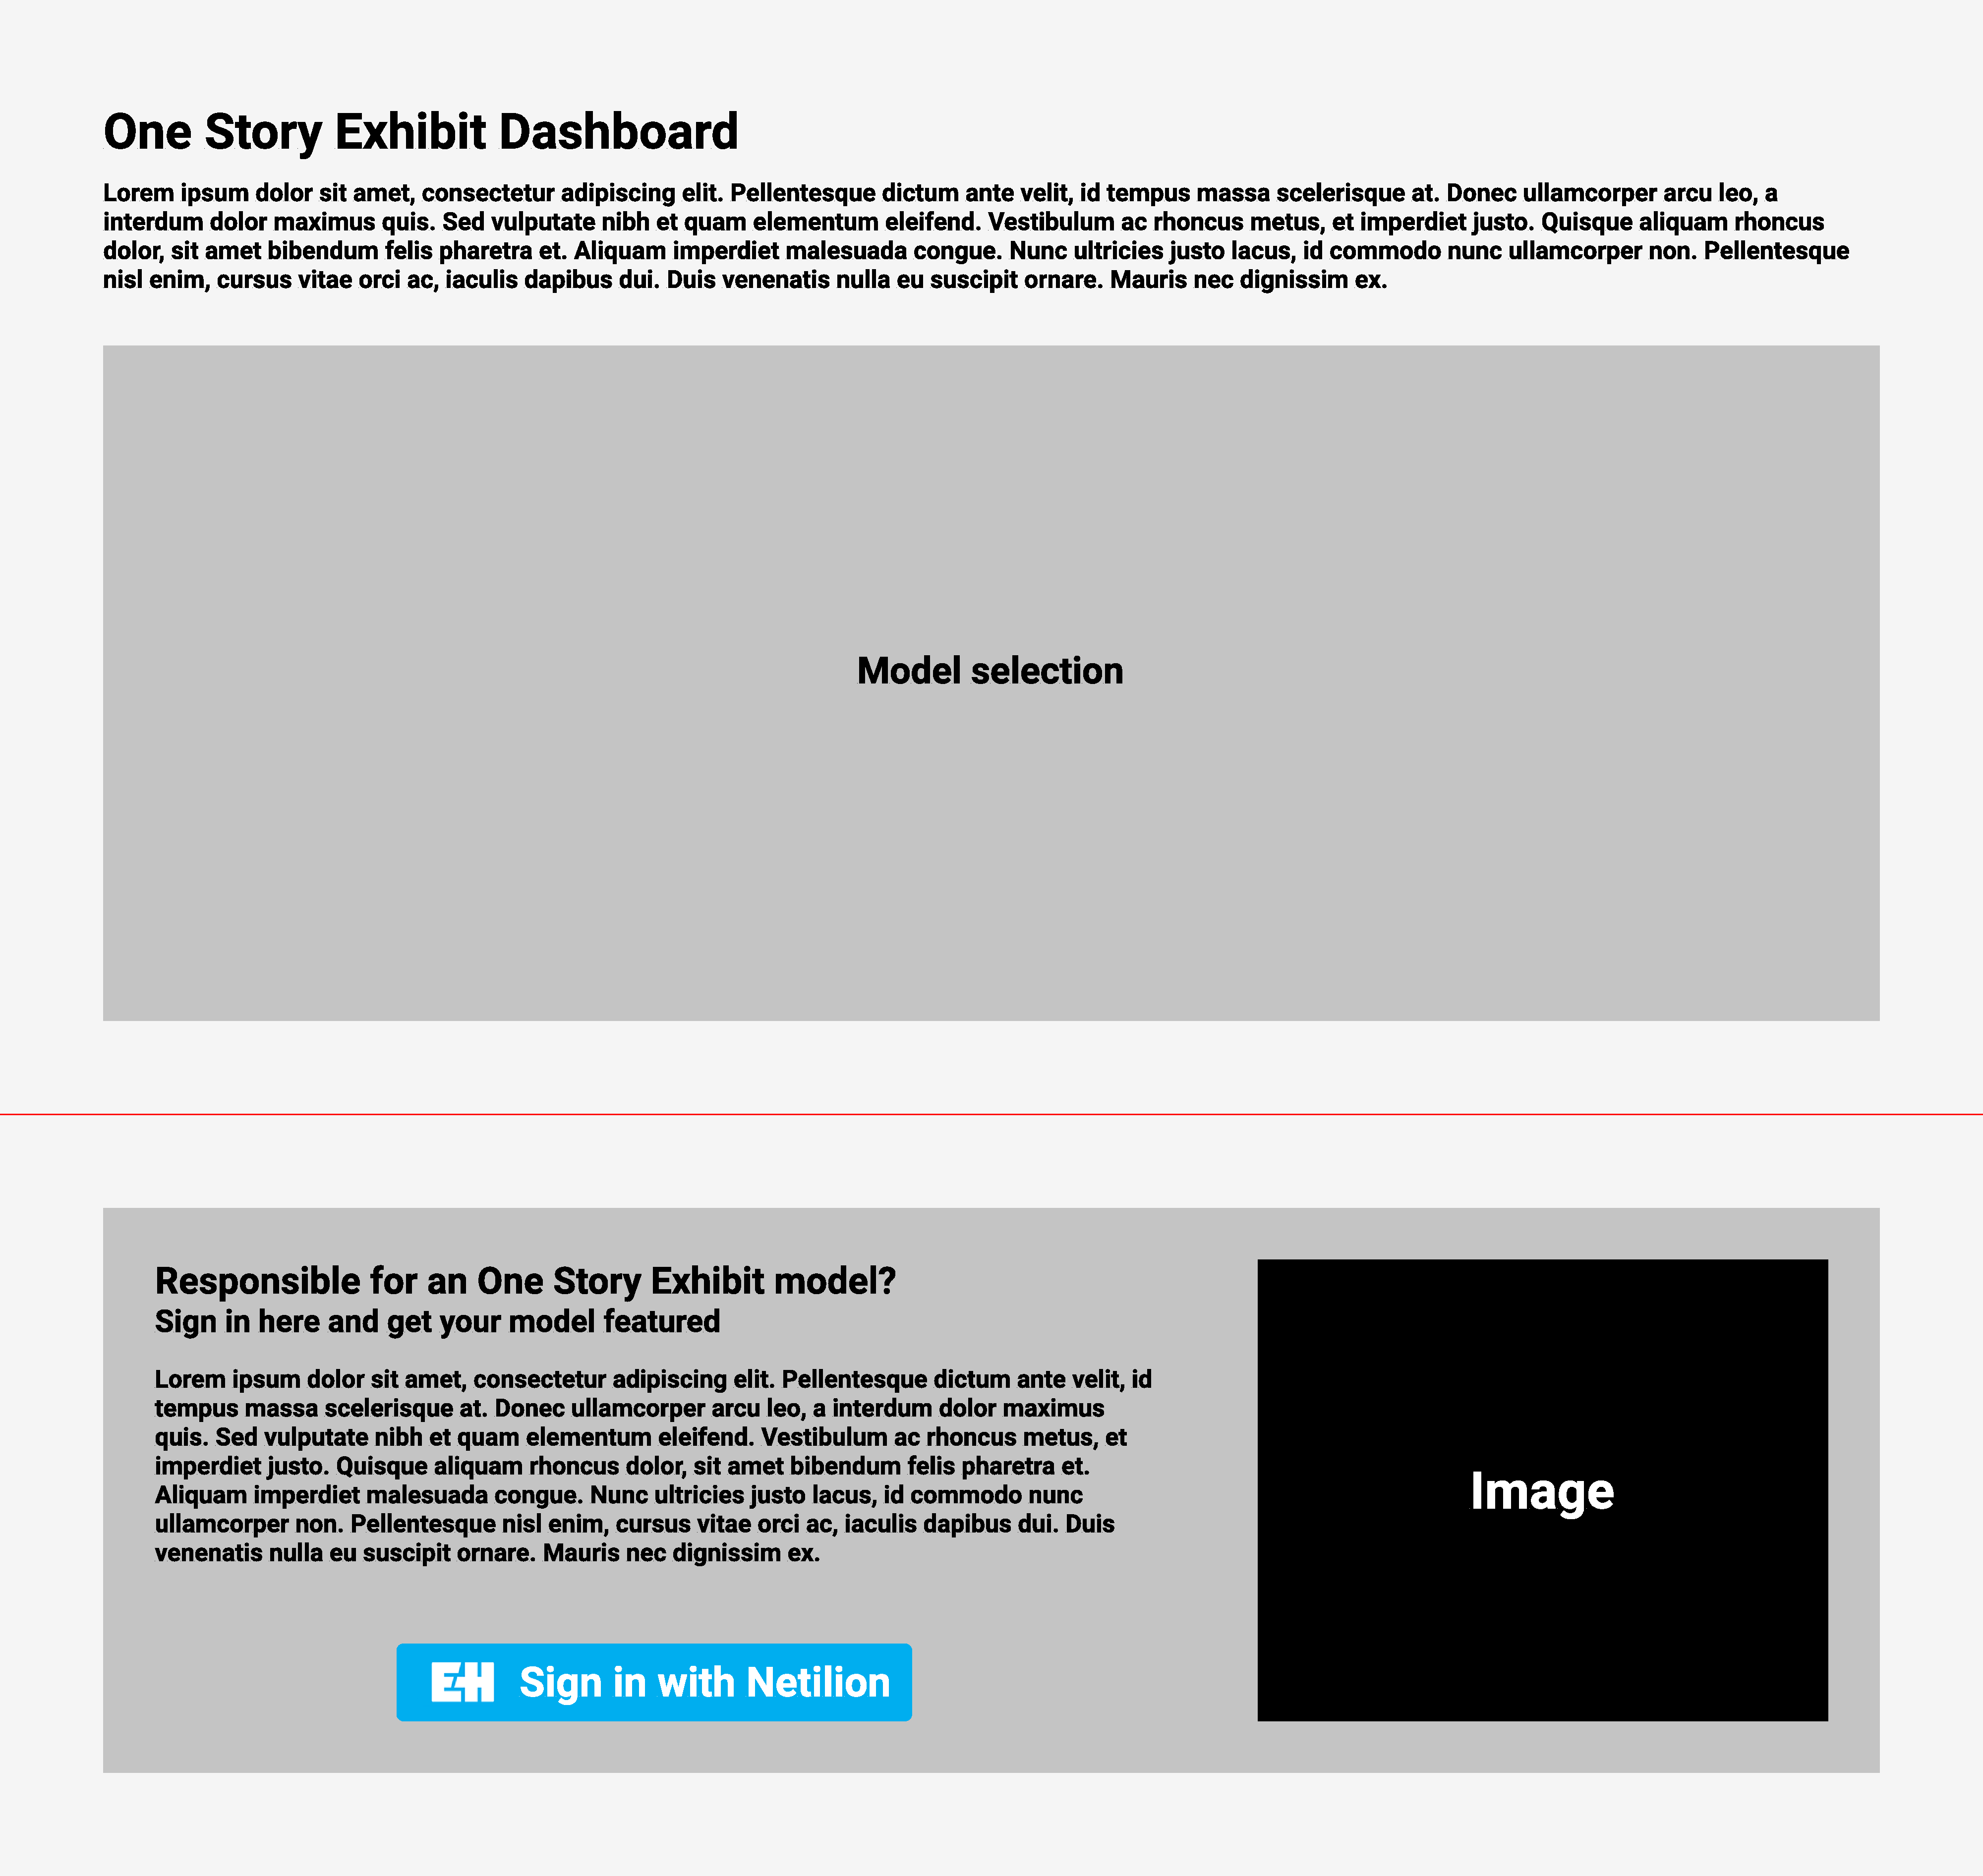
\includegraphics[width=1\textwidth]{./mockups/index/not_signed_in.pdf}
  \caption[{Mockup der Index Page}]{Mockup der Index Page}
  \label{fig:mck-index}
\end{figure}
\pagebreak
\subsection{Registration} \label{mck:registration}
\subsubsection{Fehlermeldung}
Sollte beim Loginprozess etwas schiefgehen, wird die unten dargestellte Fehlermeldung angezeigt. Dabei wird erwähnt, dass dieser Fehler sehr wahrscheinlich durch den Kandidaten geschah und nicht durch Netilion. Darunter befindet sich die Meldung, dass der User in x Sekunden wieder auf die Startseite weitergeleited wird.
\begin{figure}[H]
  \centering
  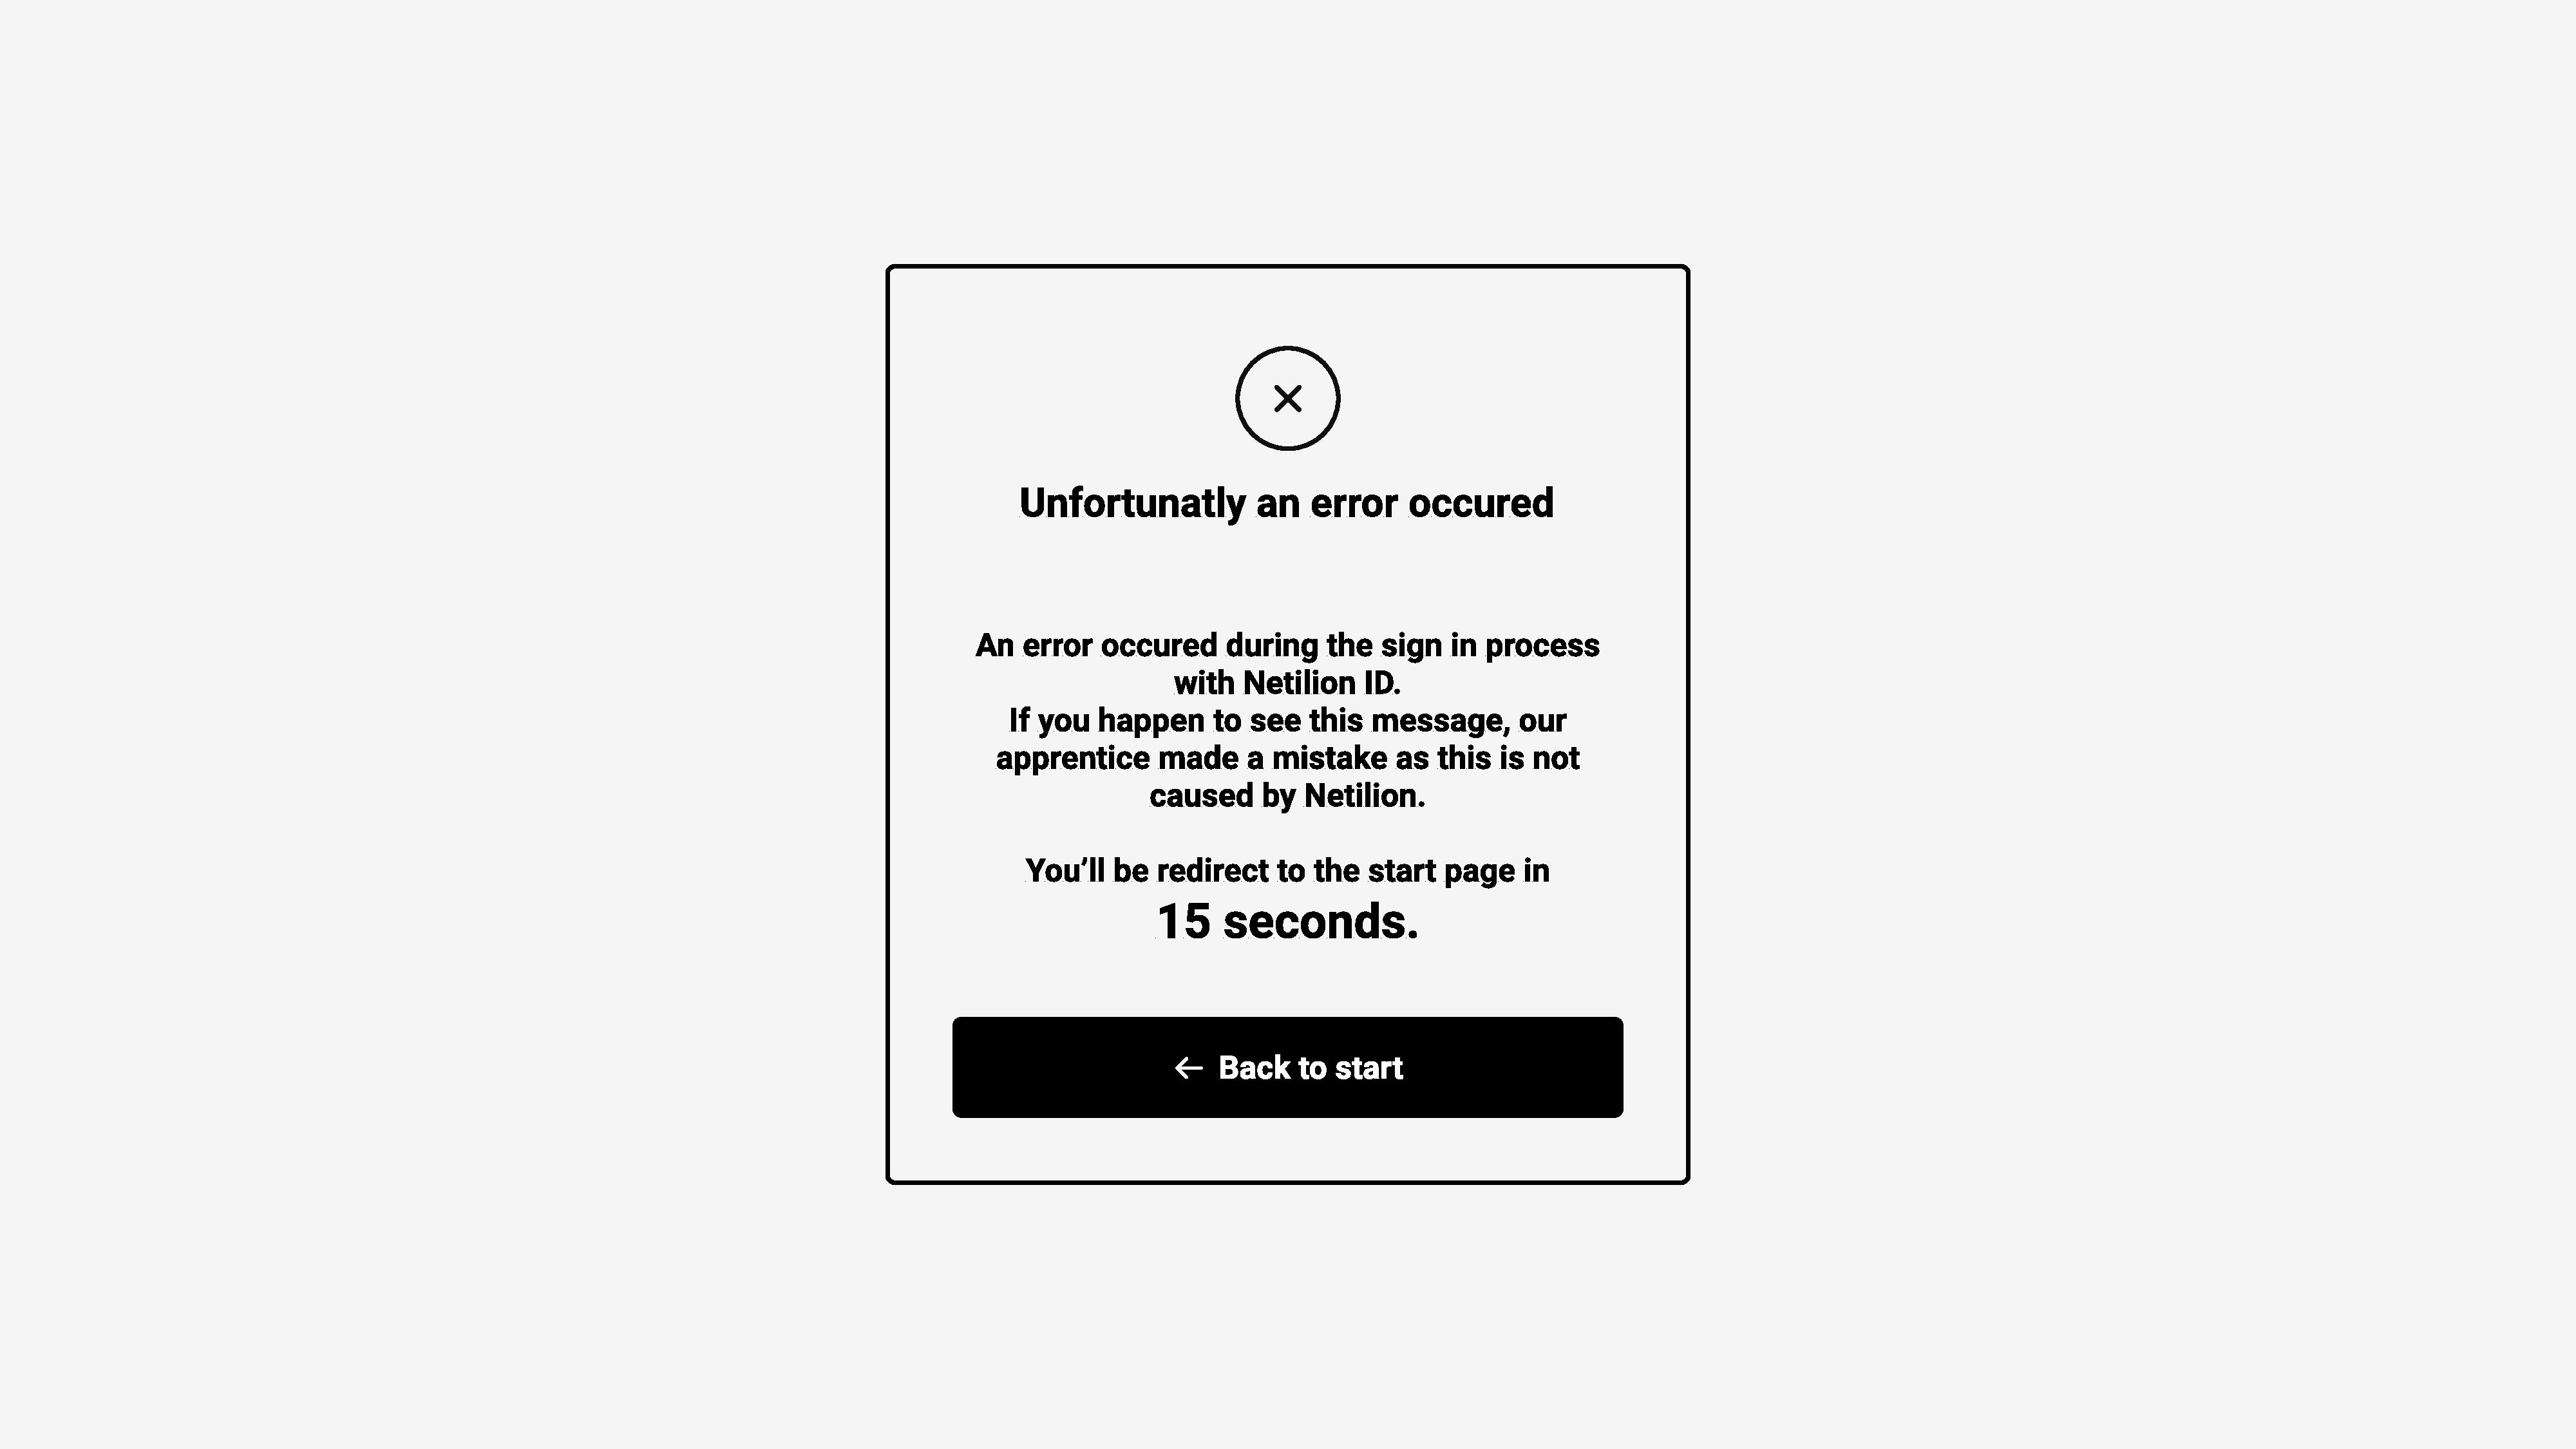
\includegraphics[width=1\textwidth]{./mockups/register/error.pdf}
  \caption[{Mockup einer Fehlermeldung}]{Mockup einer Fehlermeldung}
  \label{fig:mck-error}
\end{figure}
\pagebreak
\subsubsection{Anmeldung erfolgreich}
Diese Ansicht wird angezeigt, wenn der Loginprozess erfolgreich abläuft. Dabei wird im oberen Teil angezeigt, dass dies der Erste der insgesammt drei Schritte ist, welche für die erfolgreiche Registration benötigt werden.
\begin{figure}[H]
  \centering
  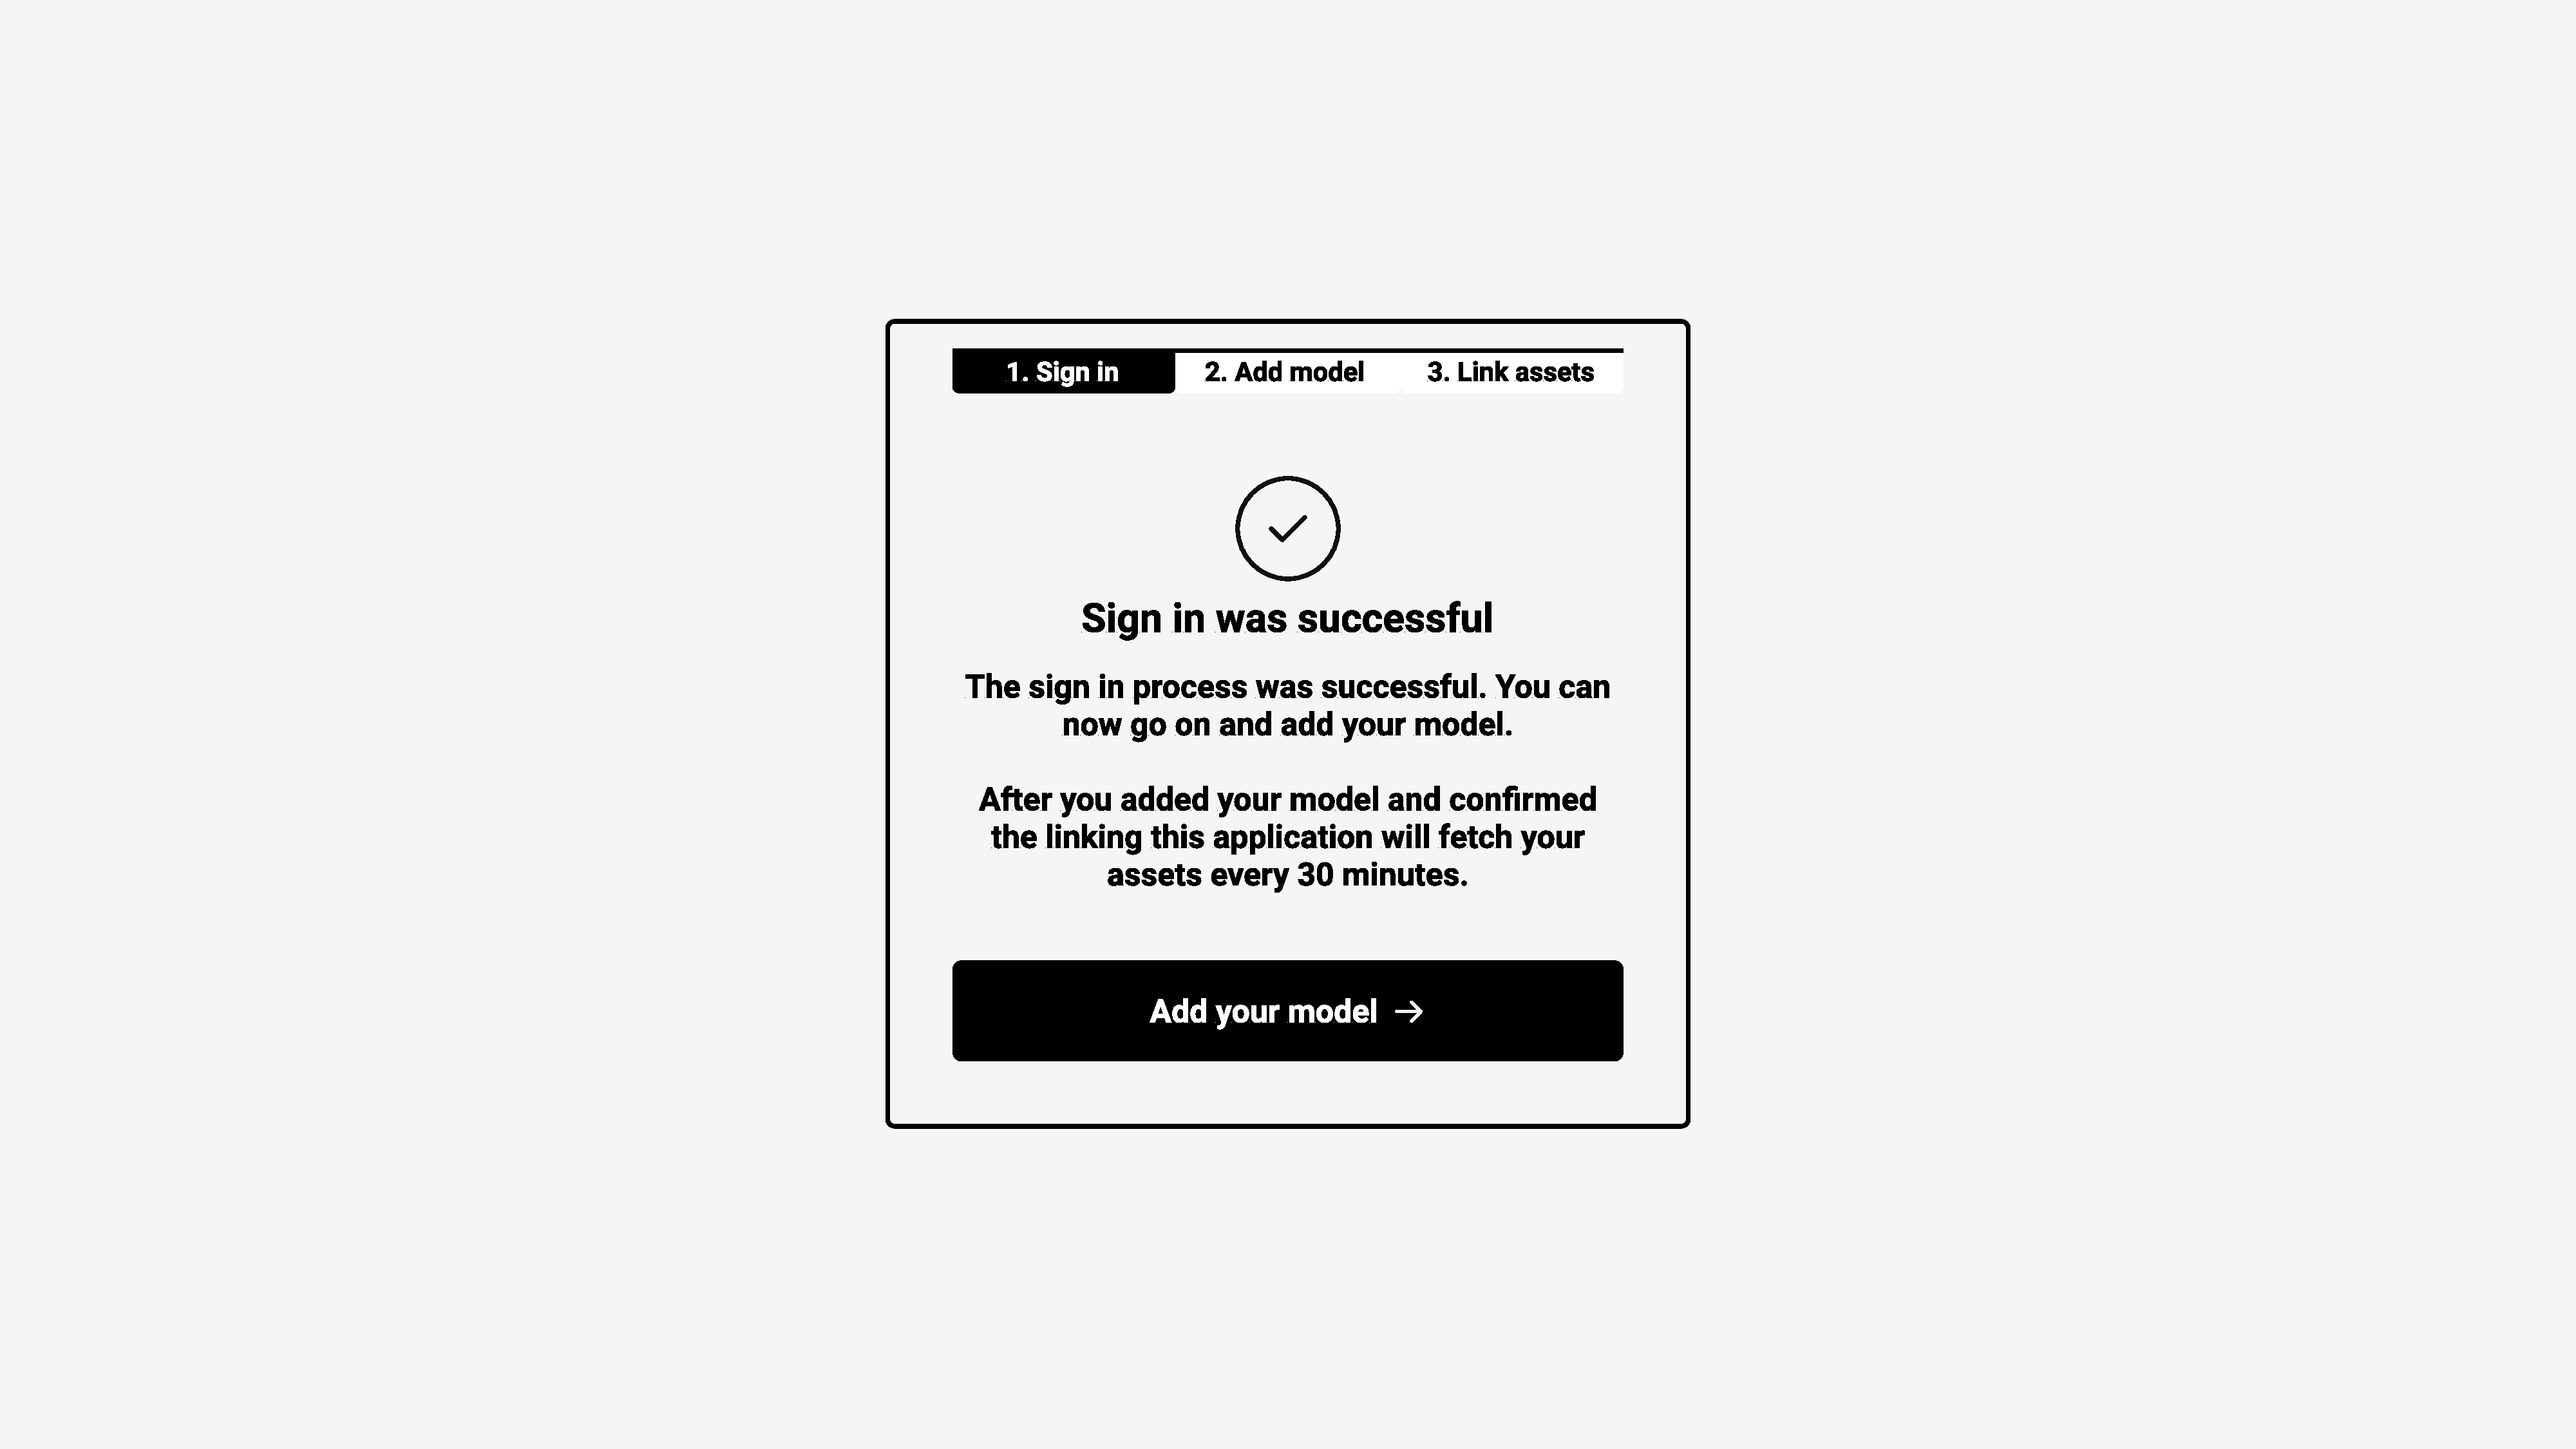
\includegraphics[width=1\textwidth]{./mockups/register/stage_1.pdf}
  \caption[{Mockup einer erfolgreichen Anmeldung}]{Mockup einer erfolgreichen Anmeldung}
  \label{fig:mck-stage_1}
\end{figure}
\pagebreak
\subsubsection{Modell registrieren}
Nun wird der OSE-Verantwortlicher darum gebeten, seinem Modell einen Namen zu geben und den Standort anzugeben, damit die User sein Modell dann über die Index Page finden können.
\begin{figure}[H]
  \centering
  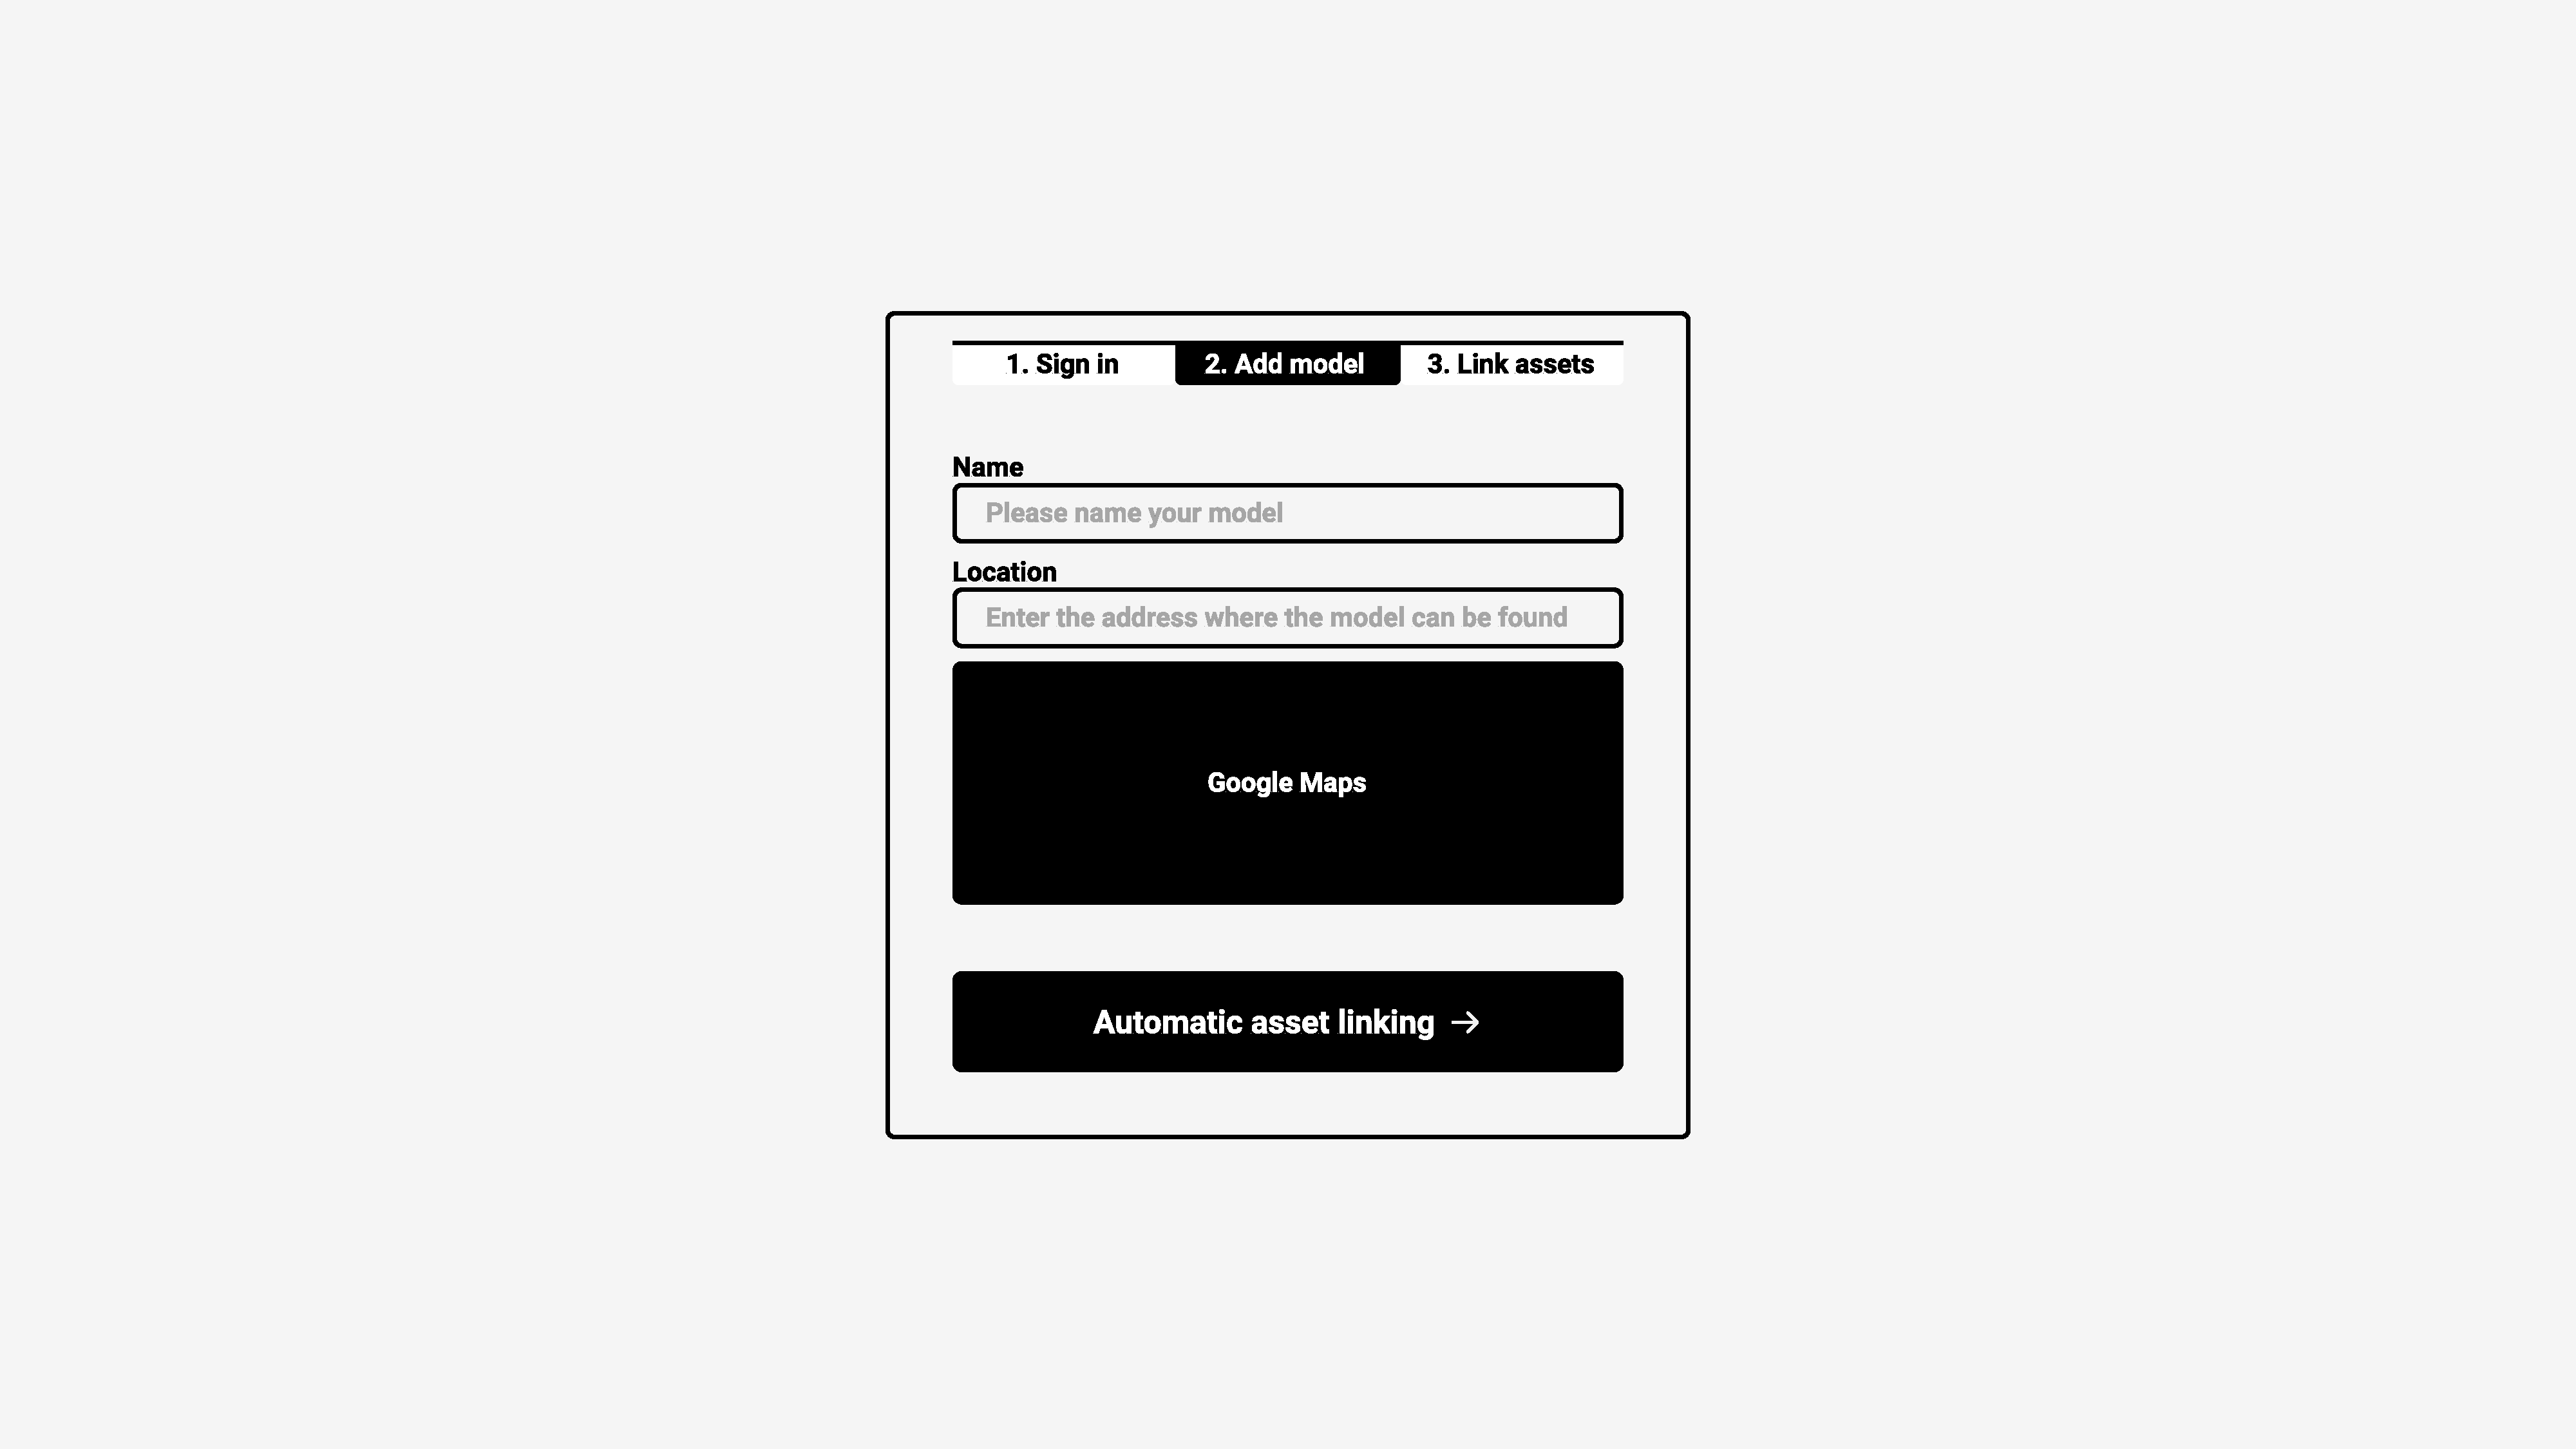
\includegraphics[width=1\textwidth]{./mockups/register/stage_2.pdf}
  \caption[{Mockup der Registration}]{Mockup der Registration}
  \label{fig:mck-stage_2}
\end{figure}
\pagebreak
\subsubsection{Asset verlinkung}
Der letzte Schritt der Registrierung ist das Verlinken der Assets mit den Meshes des 3D Modells. Da dies automatisch geschieht, wird der User an dieser stelle gebeten zu warten, bis der Prozess abgeschlossen ist.
\begin{figure}[H]
  \centering
  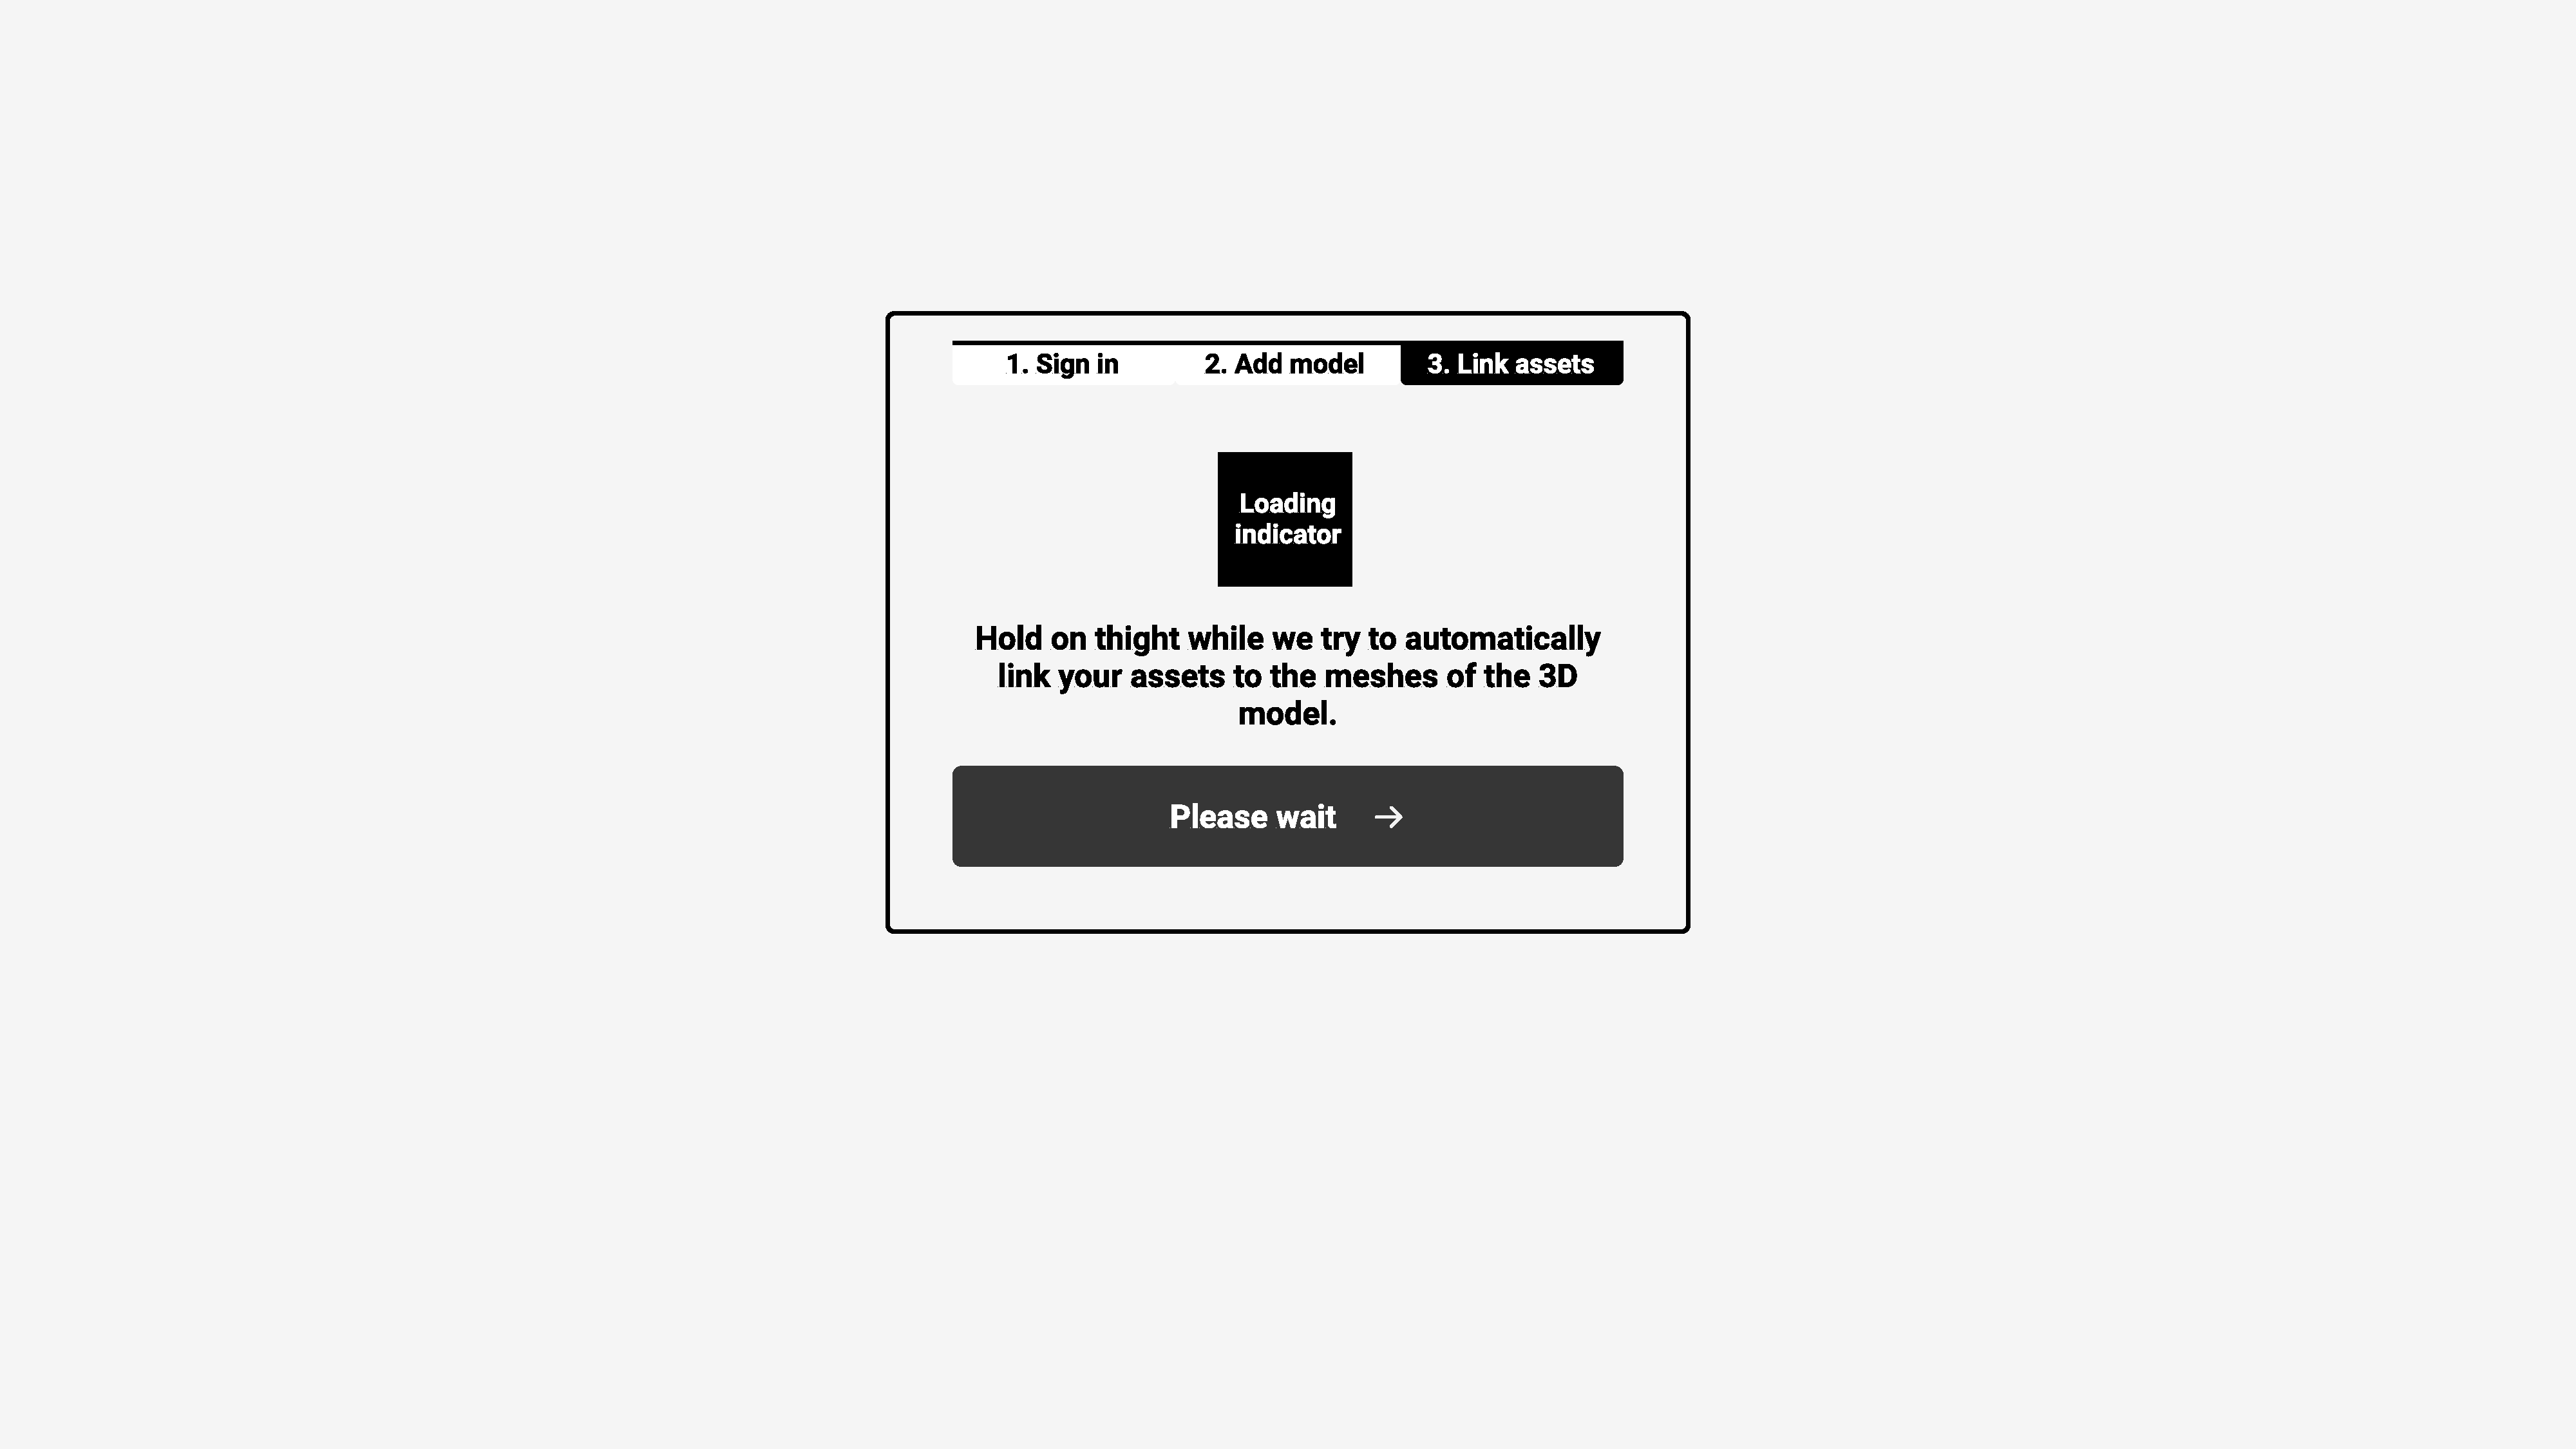
\includegraphics[width=1\textwidth]{./mockups/register/stage_3.pdf}
  \caption[{Mockup der Asset verlinkung}]{Mockup der Asset verlinkung}
  \label{fig:mck-stage_3}
\end{figure}
\pagebreak
\subsubsection{Asset verlinkung fehlgeschlagen}
Konnten nicht alle Assets verlinkt werden, wird dieses Fenster angezeigt. Es erklärt dem User was geschah und das er die Verlinkung im nächsten Schritt manuel anpassen kann.
\begin{figure}[H]
  \centering
  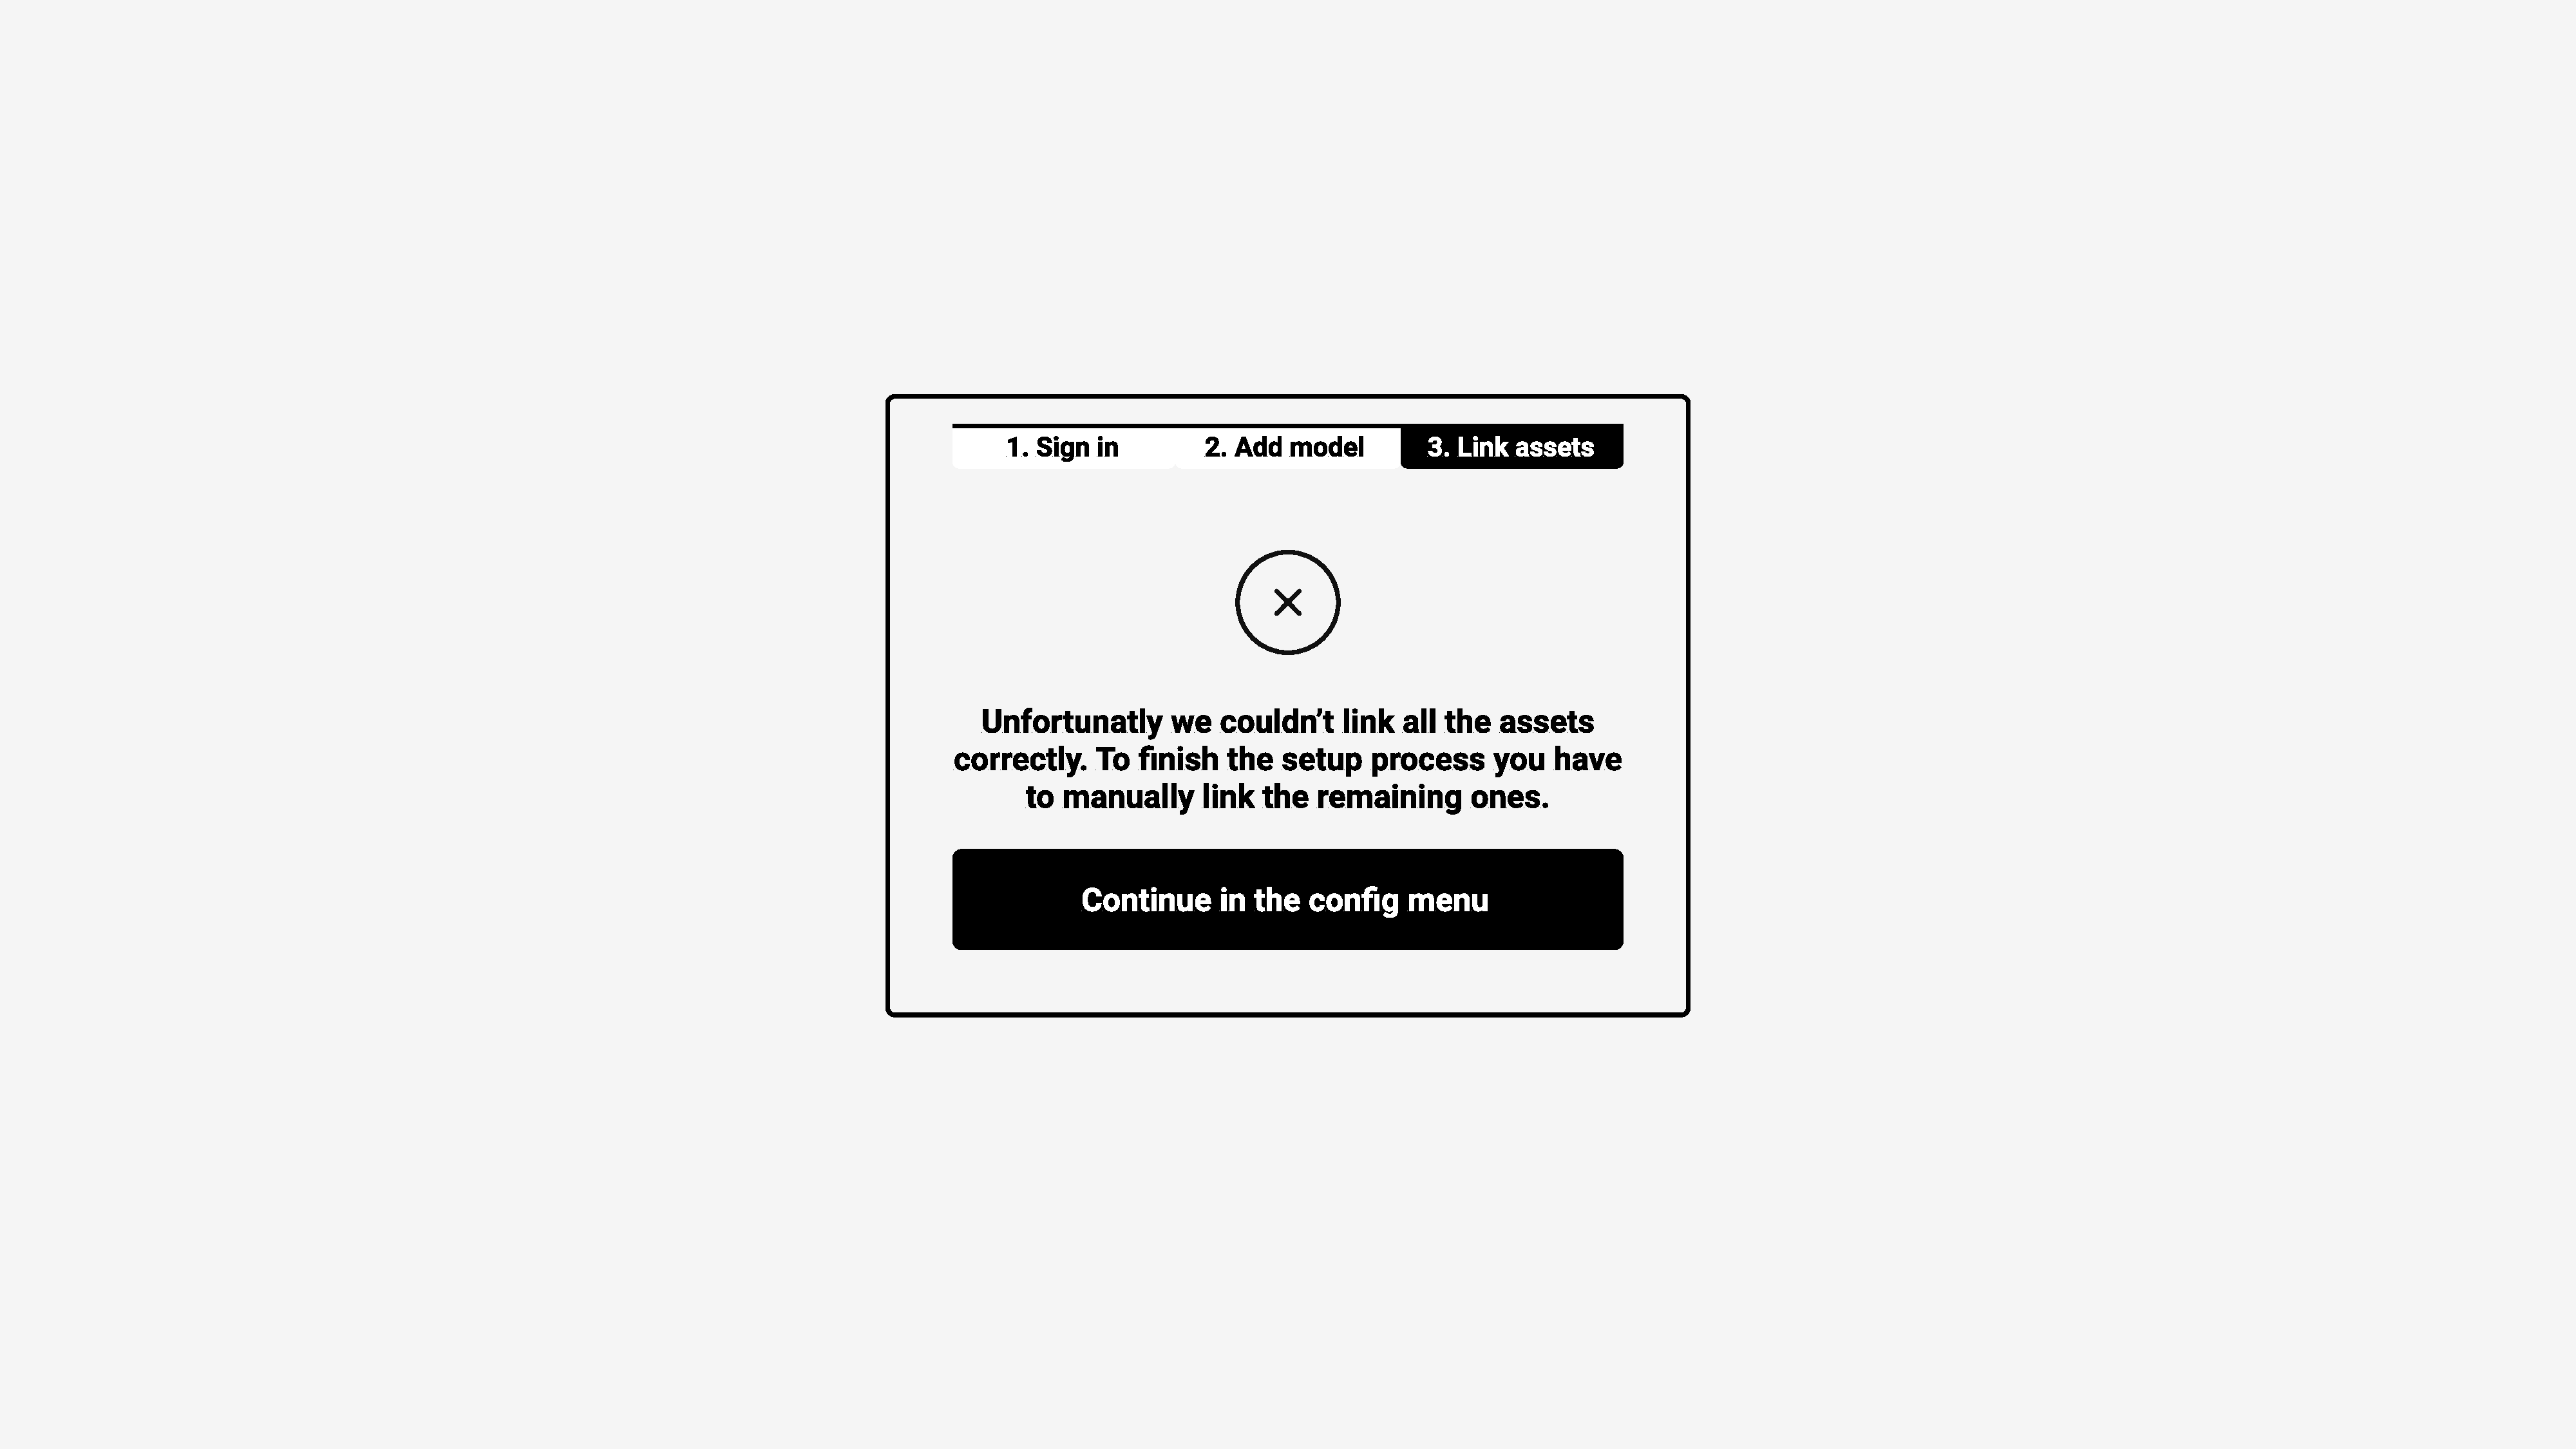
\includegraphics[width=1\textwidth]{./mockups/register/redirect.pdf}
  \caption[{Mockup einer fehlgeschlagenen Verlinkung}]{Mockup einer fehlgeschlagenen Verlinkung}
  \label{fig:mck-redirect}
\end{figure}
\pagebreak
\subsubsection{Asset verlinkung erfolgreich}
Konnten alle Assets verlinkt werden, wird dieses Fenster angezeigt. Es informiert den User, dass der Registrationsprozess hiermit abgeschlossen ist. Mit dem Knopf am unteren Rand wird er ausgeloggt und kehrt zur Startseite zurück.
\begin{figure}[H]
  \centering
  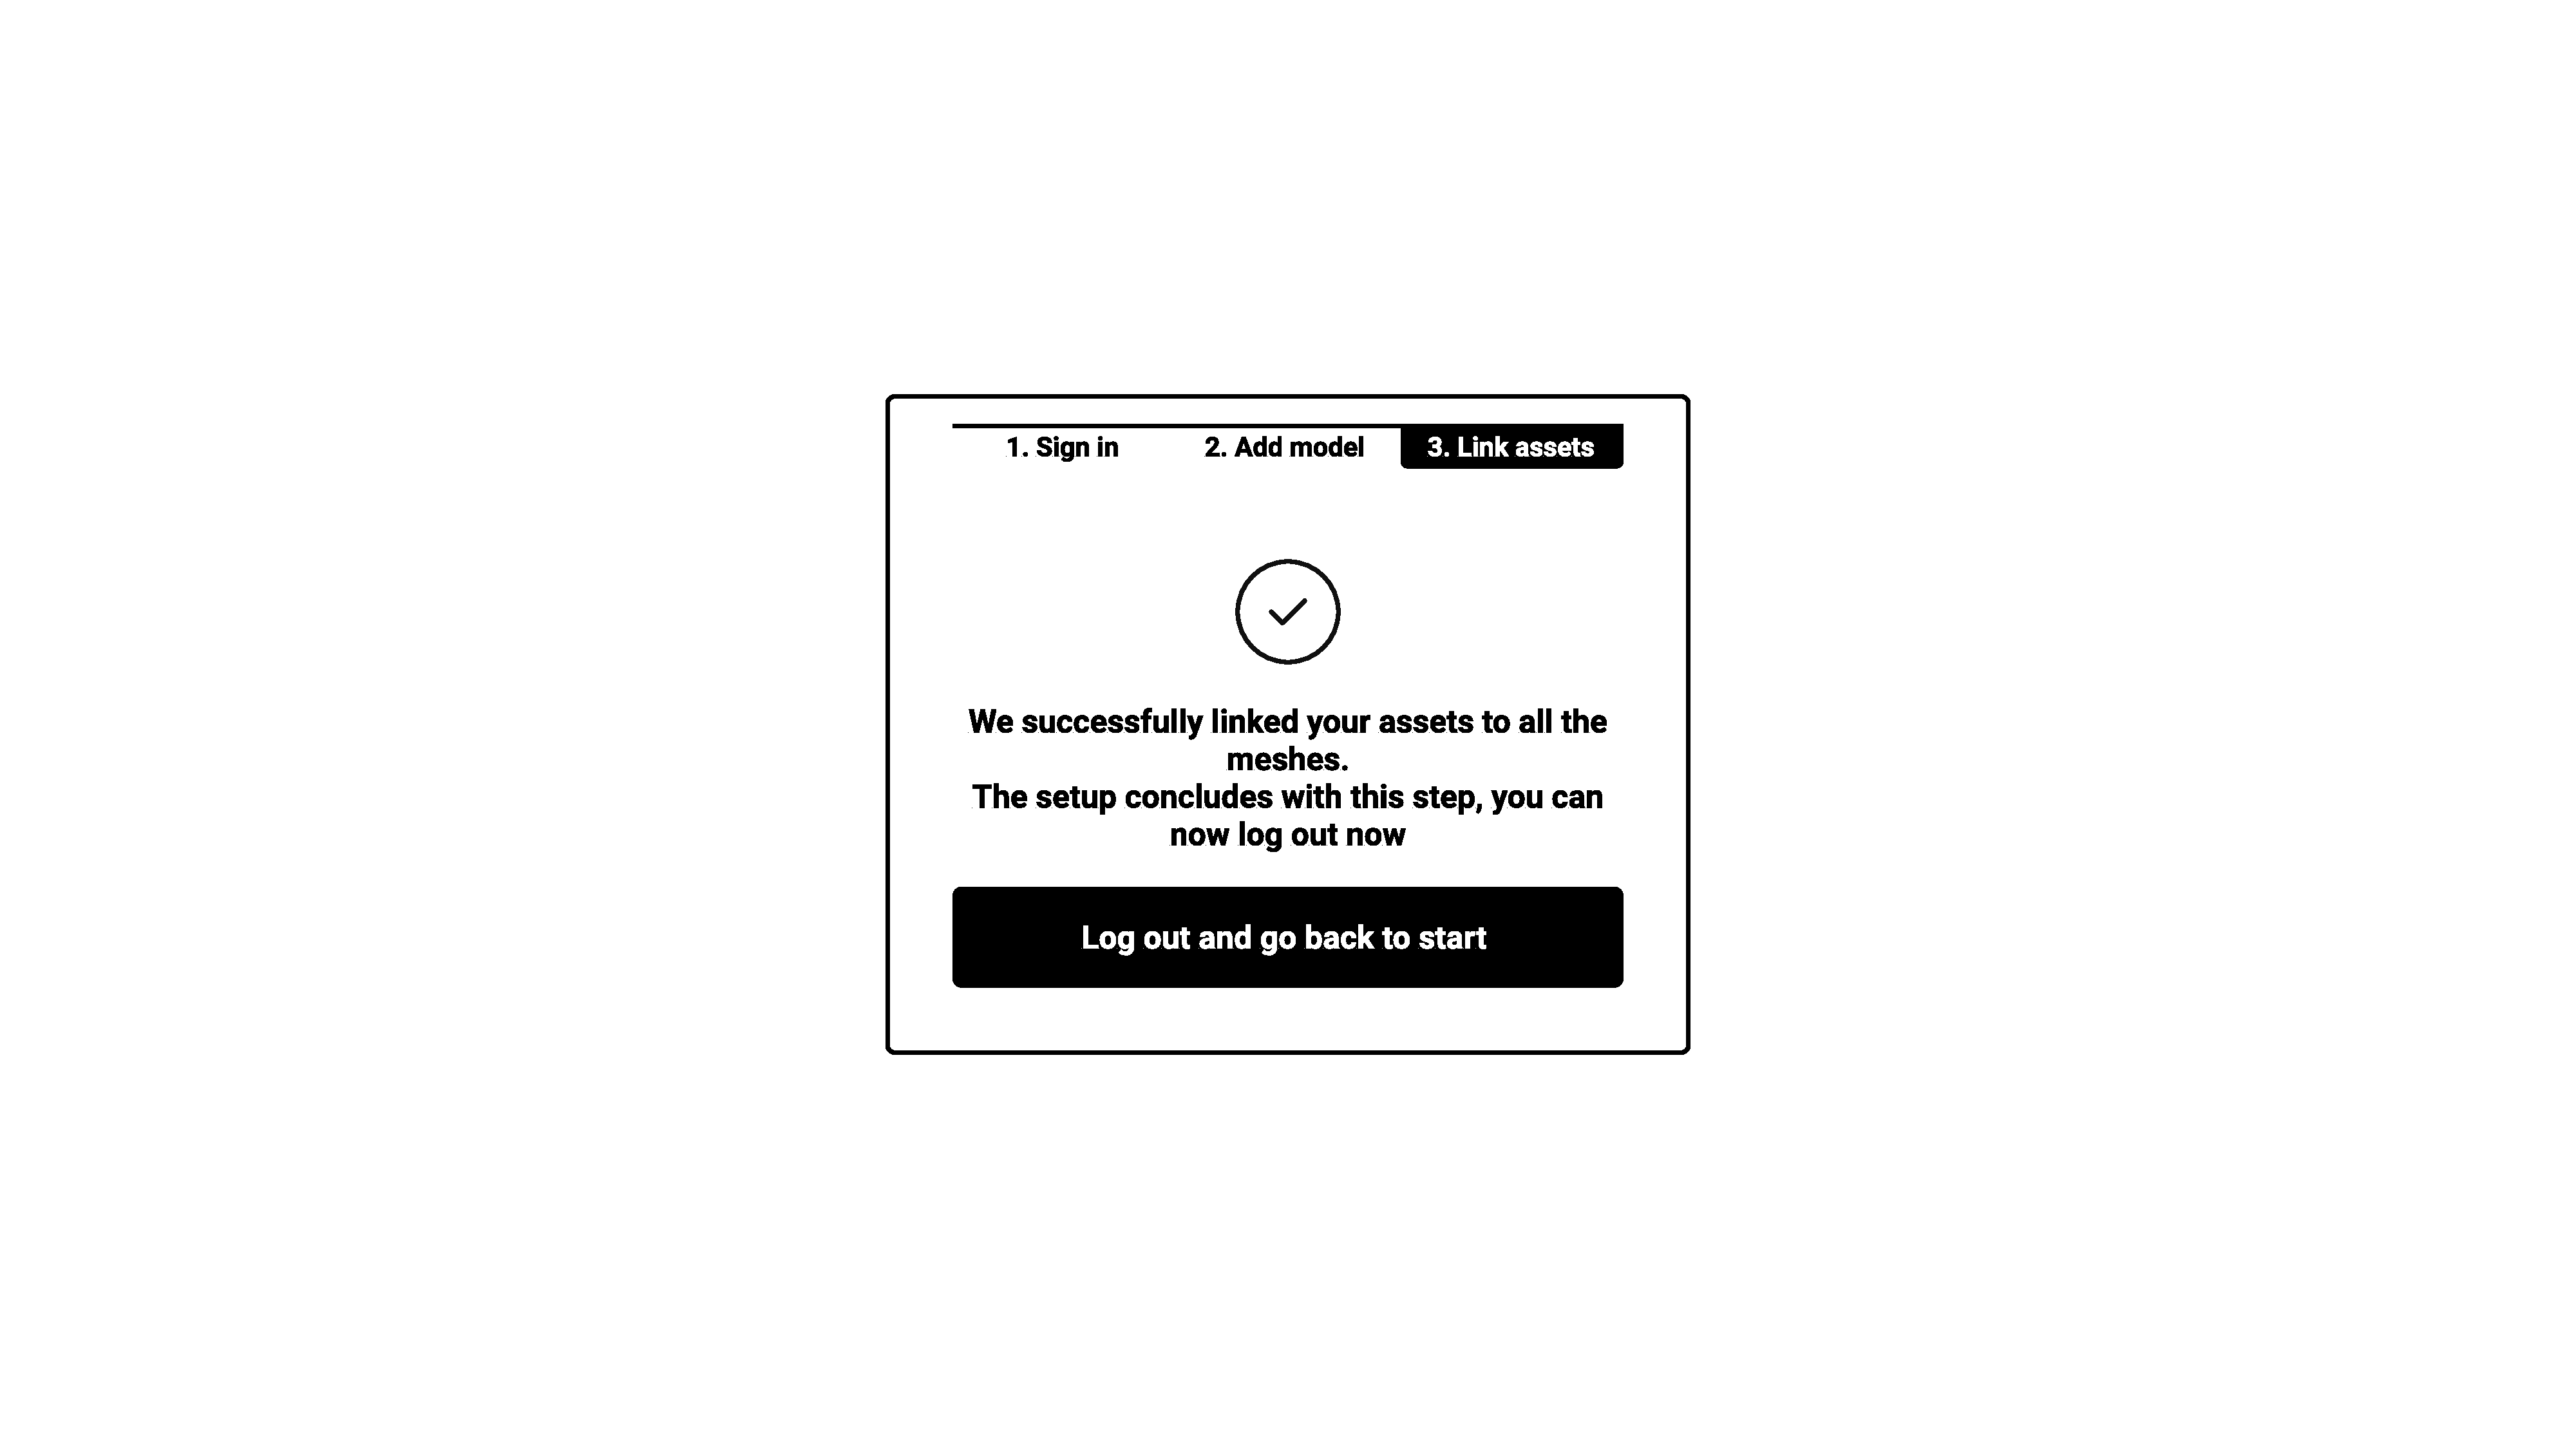
\includegraphics[width=1\textwidth]{./mockups/register/all_success.pdf}
  \caption[{Mockup einer erfolgreichen Verlinkung}]{Mockup einer erfolgreichen Verlinkung}
  \label{fig:mck-all_success}
\end{figure}
\pagebreak
\subsection{Einstellungsmenü}
\subsubsection{Modelleinstellungen}
Nachfolgend ist ein Design für die Modelleinstellungsseite. Hier kann der OSE Verantwortlicher den Namen und die Beschreibung des Modells ändern.
\begin{figure}[H]
  \centering
  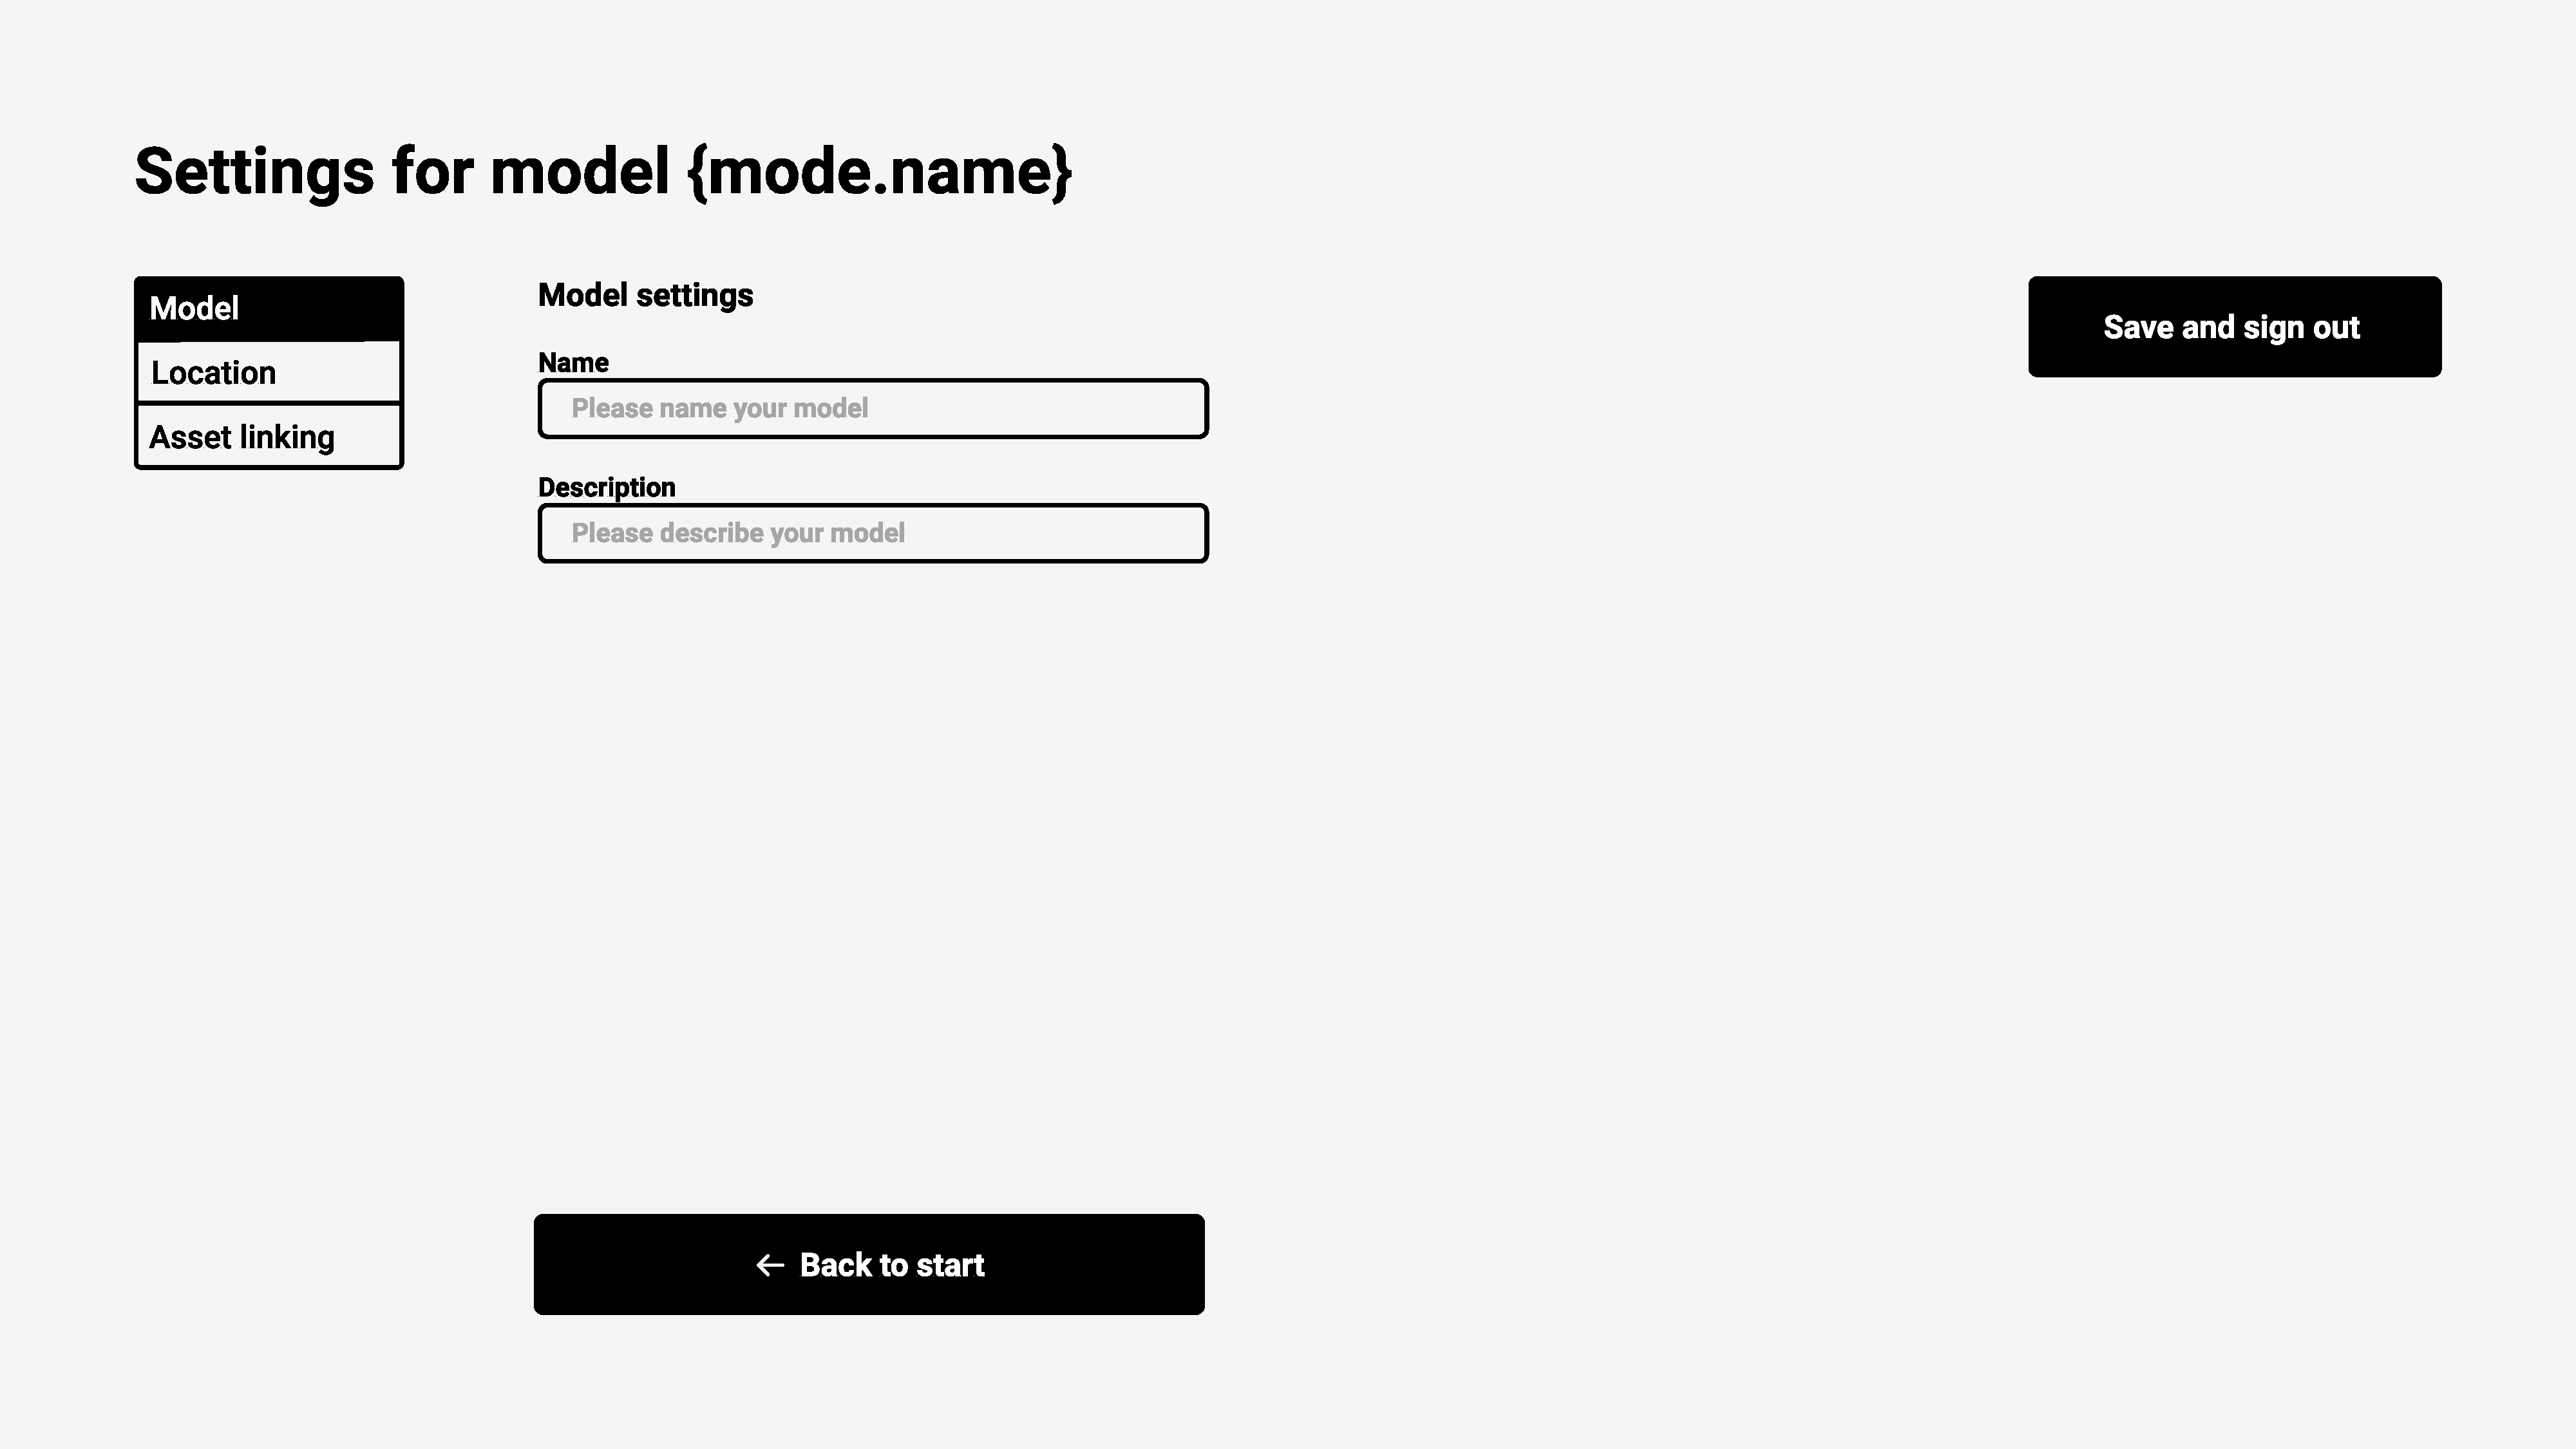
\includegraphics[width=1\textwidth]{./mockups/settings/Model.pdf}
  \caption[{Mockup des Modelleinstellungsmenü}]{Mockup des Modelleinstellungsmenü}
  \label{fig:mck-model}
\end{figure}
\pagebreak
\subsubsection{Standorteinstellungen}
Dies ist das Design für die Standortseinstellungsseite. Hier kann der Standort im nachhinein verändert werden.
\begin{figure}[H]
  \centering
  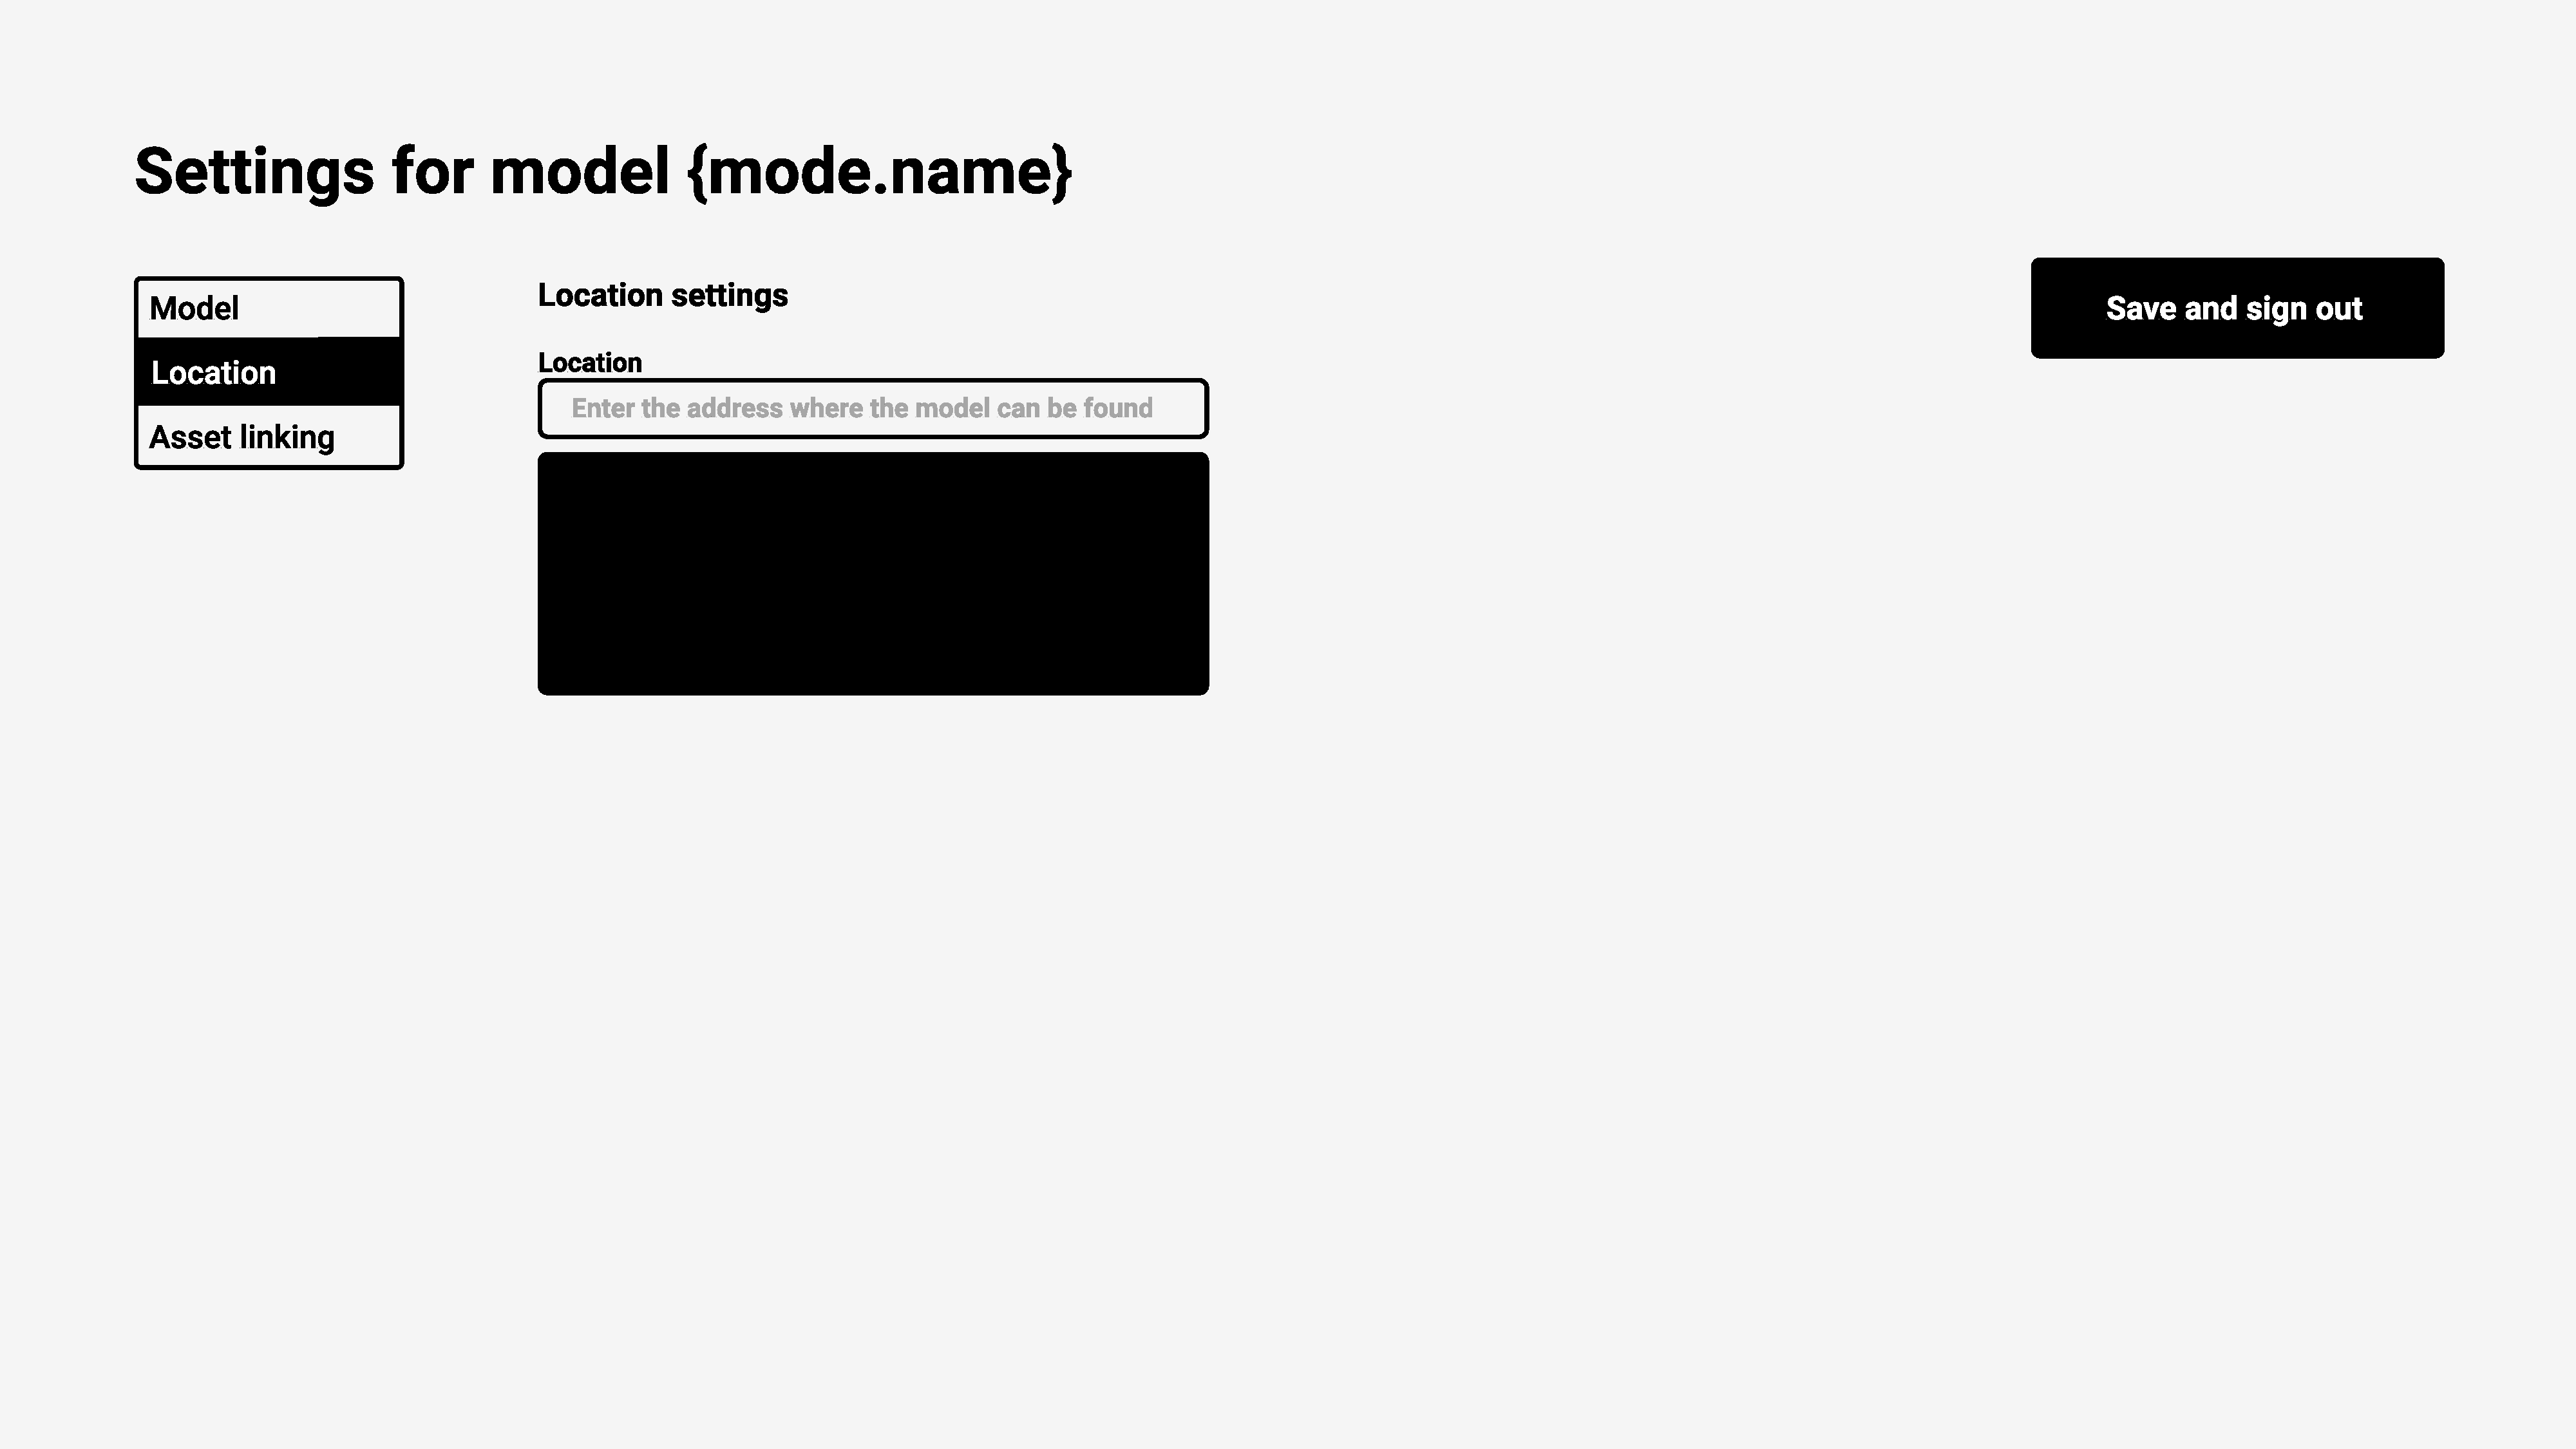
\includegraphics[width=1\textwidth]{./mockups/settings/Model-1.pdf}
  \caption[{Mockup des Standorteinstellungsmenü}]{Mockup des Standorteinstellungsmenü}
  \label{fig:mck-model_1}
\end{figure}
\pagebreak
\subsubsection{Verlinkungseinstellungen}
Nachfolgend ist ein Design für die Verlinkungseinstellungsseite. Hier kann der OSE Verantwortlicher Verlinkung des Modells ändern.
\begin{figure}[H]
  \centering
  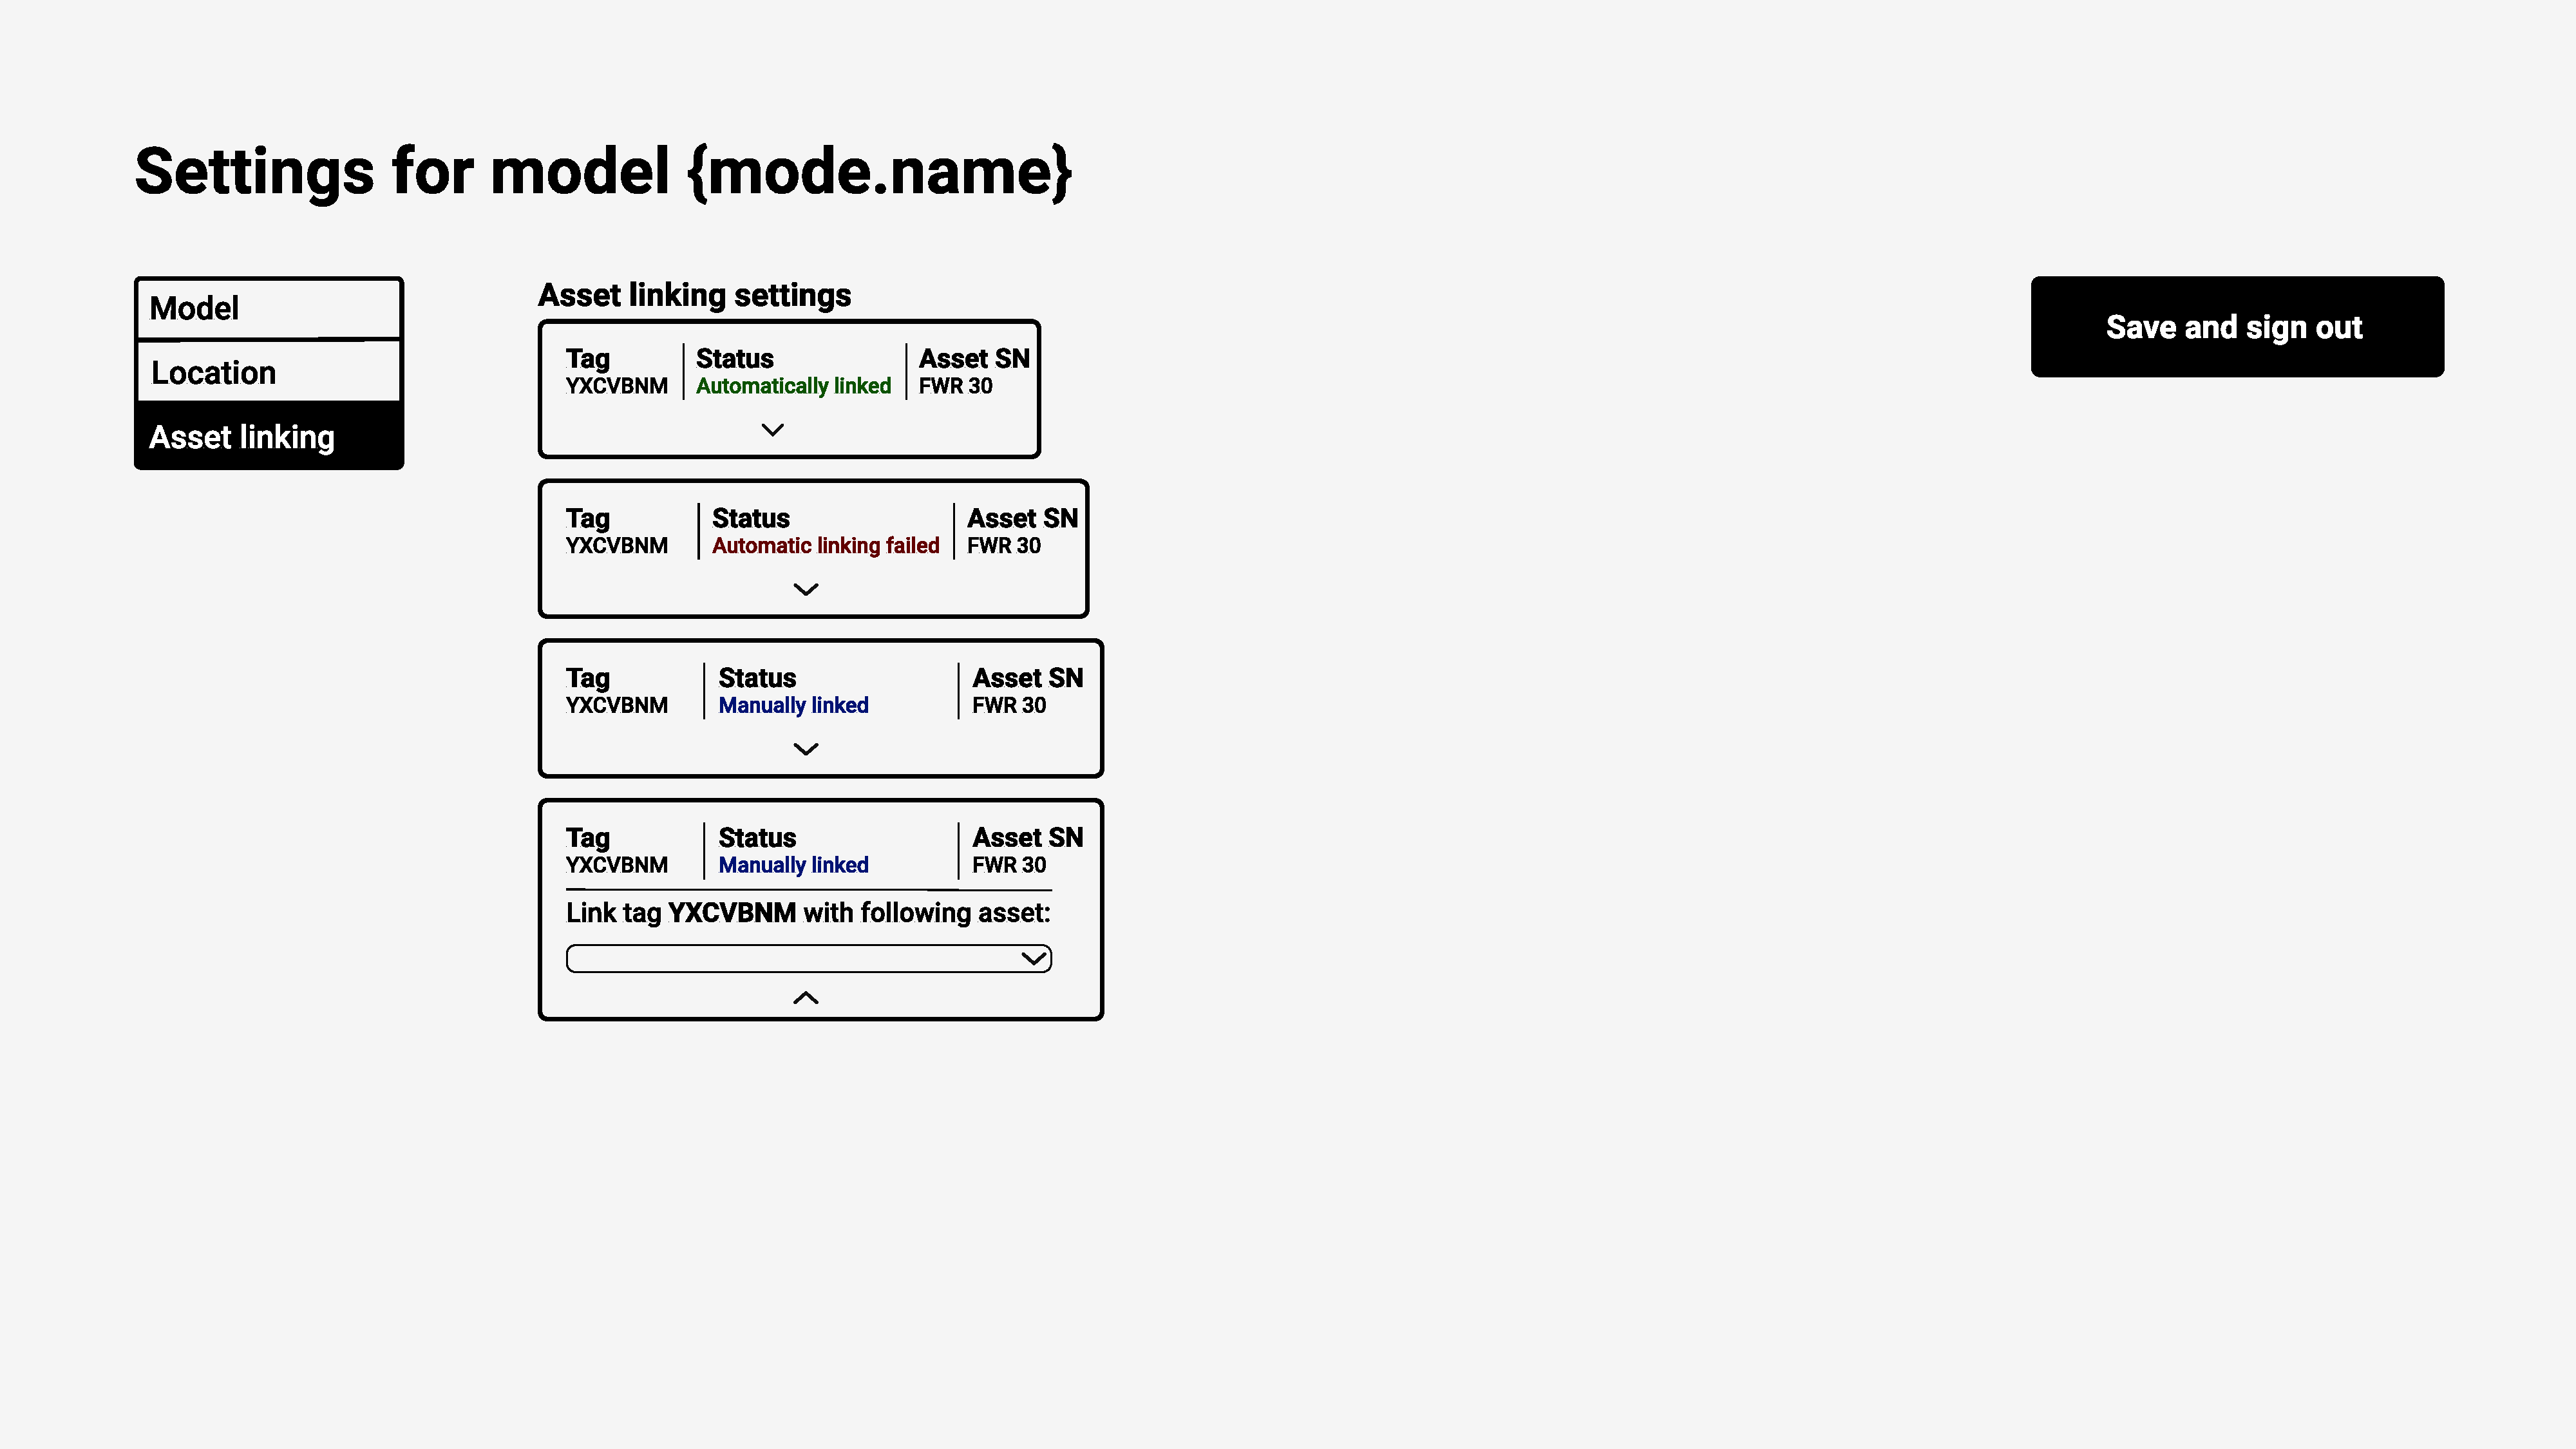
\includegraphics[width=1\textwidth]{./mockups/settings/Model-2.pdf}
  \caption[{Mockup des Verlinkungseinstellungsmenü}]{Mockup des Verlinkungseinstellungsmenü}
  \label{fig:mck-model_2}
\end{figure}
\section{Testkonzept}\label{testkonzept}
Damit sich bei der Abnahme des Projektes sicher gegangen werden kann, dass alles wie gewünscht funktioniert, wird ein Testkonzept erarbeitet. Dieses soll sich auf die bereits erstellten User-Stories stützen und so alle Anforderungen der Anspruchsgruppen abdecken. Nach der Implementierungsphase wird dieses Konzept befolgt und differenzen dokumentiert.
\newline
Einzelne Test-Cases werden wie folgt benannt:
\begin{table}[H]
  \begin{tabularx}{\textwidth}{l l X}\hline \\
  \textbf{Segment} & \textbf{Abkürzung} & \textbf{Beschreibung} \\ \\\hline \\
  1 & TC & Abkürzung für Test Case \\
  2 & - & Trennzeichen \\
  3 & 01 & Fortlaufende Kennzahl \\
  \\\hline
  \end{tabularx}
\end{table}
\subsection{Fehlerklassen}
Damit Testergebnisse nach der Prüfung priorisiert werden können, werden ihnen Fehlerklassen zugewiesen.
Fehlerklassen sind folgenderweise definiert:
\begin{table}[H]
  \begin{tabularx}{\textwidth}{l l X}\hline \\
  \textbf{Fehlerklasse} & \textbf{Beschreibung} \\ \\\hline \\
  0 & Definiertes Resultat stimmt mit dem getesteten Resultat überein \\
  1 & Definiertes Resultat weicht von dem getestet Resultat ab, beeinträchtigt die \\
    & Funktionalität allerdings nicht \\
  2 & Definiertes Resultat weicht von dem getestet Resultat ab und beeinträchtigt \\
    & die Funktionalität \\
  3 & Definiertes Resultat und getestetes Resultat stimmen nicht überein \\
  \\\hline
  \end{tabularx}
\end{table}
\subsection{Test Case Schema}
\begin{table}[H]
  \begin{tabularx}{\textwidth}{l l X}\hline \\
  \textbf{Segment} & \textbf{Beschreibung} \\ \\\hline \\
  Name & Name des Testes, gemäss des Namenskonzeptes \\
  Tester & Name der Person, die den Test durchgeführt hat \\
  Erwartetes Resultat & Vom Nutzer gewünschtes Resultat \\
  Effektives Resultat & Eingetroffenes Resultat \\
  Szenario & In Schritten definiertes Testszenario \\
  Fehlerklasse & Zugewiesene Fehlerklasse nach der Überprüfung \\
  Weiteres Vorgehen & Vorgehensbeschreibung, sollte die Fehlerklasse nicht 0 sein \\
  Status & Zeigt, ob der Test Case geprüft wurde \\
  \\\hline
  \end{tabularx}
\end{table}
\subsection{User-Stories Abdeckung}
\begin{table}[H]
  \begin{tabularx}{\textwidth}{l X l}\hline \\
  \textbf{Test-Case} & \textbf{Beschreibung} & \textbf{Betroffene User-Story} \\\hline \\
  TC-01 & Login möglich und sicher -> OAuth2konzept befolgt & US-01 \\
  TC-02 & Fehlermeldung Login & US-01 \\
  TC-03 & Automatische verlinkung Assets & US-02 \\
  TC-04 & Konfigurationsmenü aufrufbar & US-03 \\
  TC-05 & Verlinkungen manuel änderbar & US-03 \\
  TC-06 & Konfigurationsmenü nur durch eingeloggten User, welcher sich in der Usergruppe befindet, aufrufbar & US-04 \\
  TC-07 & Übersicht aller Standorte & US-06 \\
  TC-08 & Standort änderbar & US-06 \\
  \\\hline
  \end{tabularx}
\end{table}
\pagebreak
\subsection{Test-Cases}
\subsubsection{TC-01: Login}\label{tc-01}
\begin{table}[H]
  \begin{tabularx}{\textwidth}{l X}\hline \\
  Name & TC-01 \\
  Tester & Jonas Schultheiss \\
  Erwartetes Resultat & OSE Verantwortlicher kann sich anmelden \\
  Effektives Resultat & Das effektive Resultat stimmt mit dem erwarteten überein \\
  Fehlerklasse & 0 \\
  Weiteres Vorgehen & Nicht nötig \\
  Status & Durchgeführt am 13.04.2021 \\
  \\\hline
  \end{tabularx}
\end{table}
\begin{table}[H]
  \begin{tabularx}{\textwidth}{l X X}
  \textbf{Schritt} & \textbf{Beschreibung} & \textbf{Erwartetes Resultat}\\ \\\hline \\
  0 & Benutzer befindet sich auf der Startseite & / \\
  1 & Benutzer klickt den Knopf \amk{Sign in with Netilion} an & Client des Benutzers wird an Netilion ID weitergeleited \\
  2 & Benutzer gibt seine Daten an und loggt sich ein & Client des Benutzers wird zurück an das OSE-Dashboard geleited \\
  3 & Benutzer nicht registriert & Benutzer wird zur Registration weitergeleited \\
  Alternative & Benutzer registriert & Benutzer wird zum Konfigurationsmenü weitergeleited \\
  \\\hline
  \end{tabularx}
\end{table}
\pagebreak
\subsubsection{TC-02: Login falsche Logindaten}\label{tc-02}
\begin{table}[H]
  \begin{tabularx}{\textwidth}{l X}\hline \\
  Name & TC-02 \\
  Tester & Jonas Schultheiss \\
  Erwartetes Resultat & Anmeldeprozess läuft schief, aber wird bei Netilion ID direkt behandelt \\
  Effektives Resultat & Das effektive Resultat stimmt mit dem erwarteten überein \\
  Fehlerklasse & 0 \\
  Weiteres Vorgehen & Nicht nötig \\
  Status & Durchgeführt am 13.04.2021 \\
  \\\hline
  \end{tabularx}
\end{table}
\begin{table}[H]
  \begin{tabularx}{\textwidth}{l X X}
  \textbf{Schritt} & \textbf{Beschreibung} & \textbf{Erwartetes Resultat}\\ \\\hline \\
  0 & Benutzer befindet sich auf der Startseite & / \\
  1 & Benutzer klickt den Knopf \amk{Sign in with Netilion} an & Client des Benutzers wird an Netilion ID weitergeleited \\
  2 & Benutzer gibt seine Daten an und probiert sich anzumelden & Netilion ID zeigt Fehlermeldung an \\
  \\\hline
  \end{tabularx}
\end{table}
\pagebreak
\subsubsection{TC-03: Login mit unberechtigtem Account}\label{tc-03}
\begin{table}[H]
  \begin{tabularx}{\textwidth}{l X}\hline \\
  Name & TC-03 \\
  Tester & Jonas Schultheiss \\
  Erwartetes Resultat & Anmeldeprozess funktioniert und Bentzer erhält passende Fehlermeldung \\
  Effektives Resultat & Das effektive Resultat stimmt mit dem erwarteten überein \\
  Fehlerklasse & 0 \\
  Weiteres Vorgehen & Nicht nötig \\
  Status & Durchgeführt am 13.04.2021 \\
  \\\hline
  \end{tabularx}
\end{table}
\begin{table}[H]
  \begin{tabularx}{\textwidth}{l X X}
  \textbf{Schritt} & \textbf{Beschreibung} & \textbf{Erwartetes Resultat}\\ \\\hline \\
  0 & Benutzer befindet sich auf der Startseite & / \\
  1 & Benutzer klickt den Knopf \amk{Sign in with Netilion} an & Client des Benutzers wird an Netilion ID weitergeleited \\
  2 & Benutzer gibt seine Daten an und meldet sich an & Client des Benutzers wird zurück an das OSE-Dashboard geleited, wo eine passende Fehlermeldung angezeigt wird \\
  \\\hline
  \end{tabularx}
\end{table}
\pagebreak
\subsubsection{TC-04: Automatische Verlinkung der Assets}\label{tc-04}
\begin{table}[H]
  \begin{tabularx}{\textwidth}{l X}\hline \\
  Name & TC-04 \\
  Tester & Jonas Schultheiss \\
  Erwartetes Resultat & Assets und Meshes werden automatisch verlinkt \\
  Effektives Resultat & Kann ein Asset nicht mit einem Mesh verlinkt werden, bekommt dies der Nutzer nicht mit \\
  Fehlerklasse & 1 \\
  Weiteres Vorgehen & Wird in Kapitel \ref{abschluss} beschrieben \\
  Status & Durchgeführt am 13.04.2021 \\
  \\\hline
  \end{tabularx}
\end{table}
\begin{table}[H]
  \begin{tabularx}{\textwidth}{l X X}
  \textbf{Schritt} & \textbf{Beschreibung} & \textbf{Erwartetes Resultat}\\ \\\hline \\
  0 & Noch nicht registrierter Benutzer hat sich bereits angemeldet und befindet sich auf dem zweiten Tab der Registration & / \\
  1 & Benutzer geht zum nächsten Tab & Client zeigt an, dass die Verlinkung im Gange ist und Backend verlinkt die Entitäten \\
  2A & Alle Assets verlinkt & Benutzer wird benachrichtigt und kann sich ausloggen \\
  Alternative & Nicht alle Assets verlinkt & Benutzer wird benachrichtigt und kann zum Konfigurationsmenü fortfahren \\
  \\\hline
  \end{tabularx}
\end{table}
\pagebreak
\subsubsection{TC-05: Konfigurationsmenü aufrufbar}\label{tc-05}
\begin{table}[H]
  \begin{tabularx}{\textwidth}{l X}\hline \\
  Name & TC-05 \\
  Tester & Jonas Schultheiss \\
  Erwartetes Resultat & Konfigurationsmenü ist aufrufbar \\
  Effektives Resultat & Das effektive Resultat stimmt mit dem erwarteten überein \\
  Fehlerklasse & 0 \\
  Weiteres Vorgehen & Nicht nötig \\
  Status & Durchgeführt am 13.04.2021 \\
  \\\hline
  \end{tabularx}
\end{table}
\begin{table}[H]
  \begin{tabularx}{\textwidth}{l X X}
  \textbf{Schritt} & \textbf{Beschreibung} & \textbf{Erwartetes Resultat}\\ \\\hline \\
  0 & Bereits registrierter Benutzer befindet sich auf der Startseite  & / \\
  1 & Benutzer meldet sich an & Client wird zum Konfigurationsmenü weitergeleited \\
  \\\hline
  \end{tabularx}
\end{table}
\begin{table}[H]
  \begin{tabularx}{\textwidth}{l X X}
  \textbf{Schritt} & \textbf{Beschreibung} & \textbf{Erwartetes Resultat}\\ \\\hline \\
  0 & Noch nicht registrierter Benutzer befindet sich auf der Startseite  & / \\
  1 & Benutzer meldet sich an & Client wird zur Registration weitergeleited \\
  2 & Benutzer registriert sich & Client wird zum Konfigurationsmenü weitergeleited \\
  \\\hline
  \end{tabularx}
\end{table}
\pagebreak
\subsubsection{TC-06: Verlinkung manuell änderbar}\label{tc-06}
\begin{table}[H]
  \begin{tabularx}{\textwidth}{l X}\hline \\
  Name & TC-06 \\
  Tester & Jonas Schultheiss \\
  Erwartetes Resultat & Assets und Meshes werden manuell verlinkt \\
  Effektives Resultat & Das effektive Resultat stimmt mit dem erwarteten überein \\
  Fehlerklasse & 0 \\
  Weiteres Vorgehen & Nicht nötig \\
  Status & Durchgeführt am 13.04.2021 \\
  \\\hline
  \end{tabularx}
\end{table}
\begin{table}[H]
  \begin{tabularx}{\textwidth}{l X X}
  \textbf{Schritt} & \textbf{Beschreibung} & \textbf{Erwartetes Resultat}\\ \\\hline \\
  0 & Bereits registrierter Benutzer befindet sich im Konfigurationsmenü im Assets Tab  & / \\
  1 & Benutzer klickt auf eine Verlinkung & Verlinkungkomponente öffnet sich \\
  2 & Benutzer klickt auf das Dropdown & Dropdown öffnet und stellt alle verfügbaren Assets dar \\
  3 & Benutzer selektiert anderen Mesh & Knopf \amk{Save changes} wird freigeschaltet \\
  4 & Benutzer klickt Knopf & Änderungen werden gespeichert \\
  \\\hline
  \end{tabularx}
\end{table}
\pagebreak
\subsubsection{TC-07: Übersicht aller Standorte}\label{tc-07}
\begin{table}[H]
  \begin{tabularx}{\textwidth}{l X}\hline \\
  Name & TC-07 \\
  Tester & Jonas Schultheiss \\
  Erwartetes Resultat & Benutzer sieht übersicht aller Standorte \\
  Effektives Resultat & Das effektive Resultat stimmt mit dem erwarteten überein \\
  Fehlerklasse & 0 \\
  Weiteres Vorgehen & Nicht nötig \\
  Status & Durchgeführt am 13.04.2021 \\
  \\\hline
  \end{tabularx}
\end{table}
\begin{table}[H]
  \begin{tabularx}{\textwidth}{l X X}
  \textbf{Schritt} & \textbf{Beschreibung} & \textbf{Erwartetes Resultat}\\ \\\hline \\
  0 & Benutzer befindet sich auf der Startseite  & / \\
  1 & Benutzer öffnet die Augen & Benutzer sieht auf der initialen Ansicht der Startseite die Standortauswahl \\
  \\\hline
  \end{tabularx}
\end{table}
\pagebreak
\subsubsection{TC-08: Standort änderbar}\label{tc-08}
\begin{table}[H]
  \begin{tabularx}{\textwidth}{l X}\hline \\
  Name & TC-08 \\
  Tester & Jonas Schultheiss \\
  Erwartetes Resultat & Standort ist änderbar \\
  Effektives Resultat & Das effektive Resultat stimmt mit dem erwarteten überein \\
  Fehlerklasse & 0 \\
  Weiteres Vorgehen & Nicht nötig \\
  Status & Durchgeführt am 13.04.2021 \\
  \\\hline
  \end{tabularx}
\end{table}
\begin{table}[H]
  \begin{tabularx}{\textwidth}{l X X}
  \textbf{Schritt} & \textbf{Beschreibung} & \textbf{Erwartetes Resultat}\\ \\\hline \\
  0 & Bereits registrierter Benutzer befindet sich auf der Startseite  & / \\
  1 & Benutzer meldet sich an & Benutzer wird angemeldet und zum Konfigurationsmenü weitergeleitet \\
  2 & Benutzer klickt auf den Tab \amk{Location} & Benutzer wird zu \code{/settings/location} weitergeleitet \\
  3 & Benutzer gibt im Eingabefeld eine neue Addresse ein & Passende Adressen wird automatisch werden vorgeschlagen \\
  4 & Benutzer klickt auf einen Adressensvorschlag & Adresse wird im Eingabefeld vervollständigt \\
  5 & Benutzer klickt auf den Knopf \amk{Save changes} & Änderungen werden gespeichert \\
  \\\hline
  \end{tabularx}
\end{table}
\pagebreak
\section{Datenbankerweiterung}
Damit die gewünschten Änderungen implementiert werden können, muss die Datenbank erweitert werden. Die Änderungen sind in der Abbildung \ref{fig:db-erweiterung} grün dargestellt. Grau markierte Tabellen sind bereits bestehende Elemente, welche in der Vorarbeit implementiert wurden.
\begin{figure}[H]
  \centering
  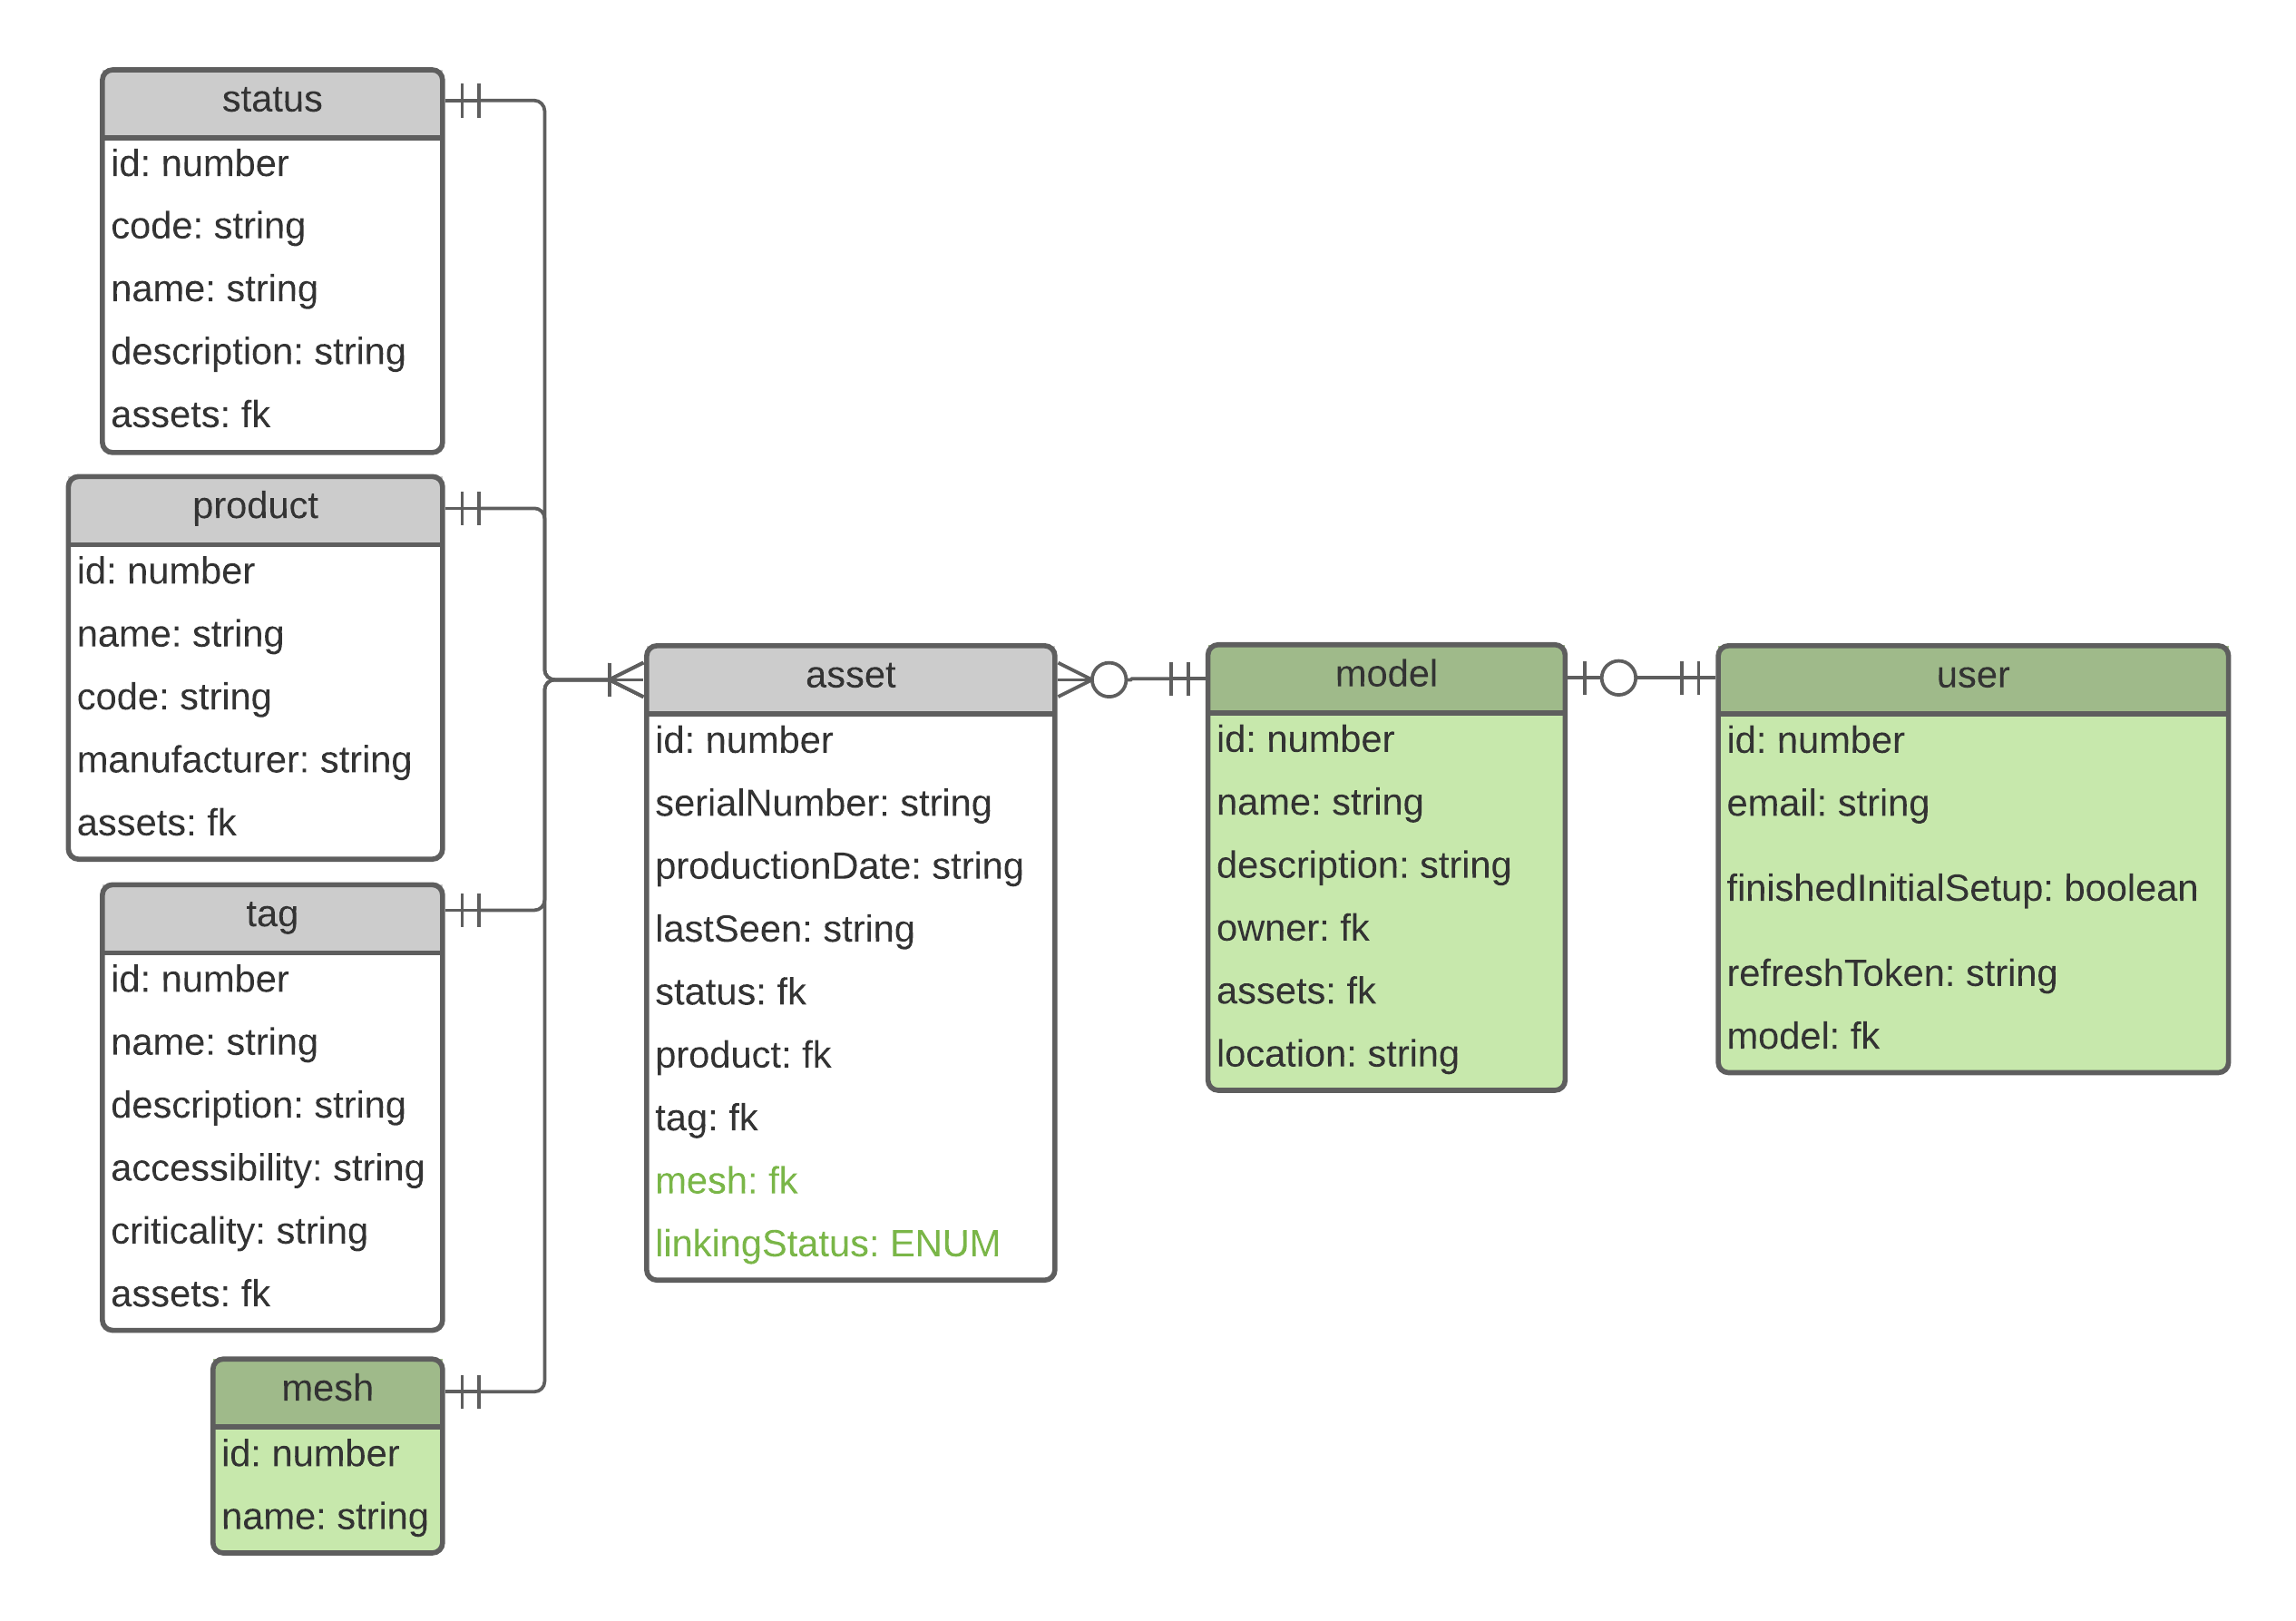
\includegraphics[width=.95\linewidth]{./images/ERM-OSE.png}
  \caption[{ERM welches die Datenbankerweiterung visualisiert}]{ERM welches die Datenbankerweiterung visualisiert}
  \label{fig:db-erweiterung}
\end{figure}
\subsection{User}
Die Userentität hat drei verwendungen:
\begin{itemize}
  \item Soll zu einem JWT geformt werden, welcher zur authentifizierung verwendet werden soll
  \item Soll den \code{refresh\_token} speichern
  \item Soll speichern, ob der User die Registration abgeschlossen hat
\end{itemize}
\subsection{Model}
Das Modell soll einen Namen und eine Beschreibung enthalten. Diese Angaben können später verwendet werden, wenn das jeweilige Modell angezeigt wird. Das Attribut \amk{location} enthält eine Id, mit welcher die genaue Adresse und Koordinaten beim Backend angefragt werden können. Ausserdem dient das Modell als Bindeglied zwischen dem \amk{User} und den \amk{Assets}.
\subsection{Mesh}
Das Mesh wird wird verwendet um die Verlinkung zwischen dem 3D-Modell und dem einzelnen Asset zu ermöglichen. Das Mesh selbst enthält dabei nur einen Namen. Bei der Planung dieser IPA wurde nicht beachtet, dass die Namen der Meshes hinzugefügt werden müssen. Da es keinen Administrator in der Applikation gibt und Nestjs, beziehungsweise das darunterliegende ORM TypeOrm, kein Seeding unterstützt, müssen diese Daten manuel der Datenbank hinzugefügt werden. Im Repository des Backends soll ein SQL und ein CSV hinterlegt werden, womit die Daten dann mit Postico, einem PostgreSQL Client, hinzugefügt werden können.
\newline
Damit das Frontend auch anzeigen kann, ob ein Asset nun automatisch oder manuell verlinkt wurde, soll der Assetentität ein enum mit dem Namen \amk{linkingStatus} hinzugefügt werden. Dieses enum soll folgende Auswahl zur verfügung stellen:
\begin{itemize}
  \item Nicht verlinkt
  \item Automatisch verlinkt
  \item Automatische Verlinkung schlug fehl
  \item Manuell verlinkt
\end{itemize}
\section{Authentifizierung mit JWT}
Die Authentifizierung zwischen dem Front- und Backend, wird mit \amk{JSON Web Tokens} gelöst. Dies wurde vom Kandidaten in einigen vorherigen Arbeiten so angewendet und ist für Ihn der Standard, wenn die Schichten getrennt werden.
\subsection{Was ist ein JWT}
\amk{JSON Web Token (JWT) ist ein offener Standard (RFC 7519), der eine kompakte und in sich geschlossene Methode zur sicheren Übertragung von Informationen zwischen Parteien als JSON-Objekt definiert. Diese Informationen können verifiziert und vertrauenswürdig sein, da sie digital signiert sind. JWTs können mit einem Geheimnis (mit dem HMAC-Algorithmus) oder einem öffentlichen/privaten Schlüsselpaar mit RSA oder ECDSA signiert werden.
\newline
Obwohl JWTs auch verschlüsselt werden können, um die Geheimhaltung zwischen den Parteien zu gewährleisten, werden wir uns auf signierte Token konzentrieren. Signierte Token können die Integrität der darin enthaltenen Ansprüche verifizieren, während verschlüsselte Token diese Ansprüche vor anderen Parteien verbergen. Wenn Token mit öffentlichen/privaten Schlüsselpaaren signiert werden, bescheinigt die Signatur auch, dass nur die Partei, die den privaten Schlüssel besitzt, diejenige ist, die sie signiert hat.}\cite{auth0.com}.
\newline
\newline
Ein JWT besteht aus drei Bestandteilen: dem Header, der Payload und der Signatur. Der Header enthält den Algorithmus mit dem der JWT encoded wird und den Typ des Tokens. Der Payload kann von der Applikation selbst bestimmt werden, sollte allerdings klein gehalten werden, da der JWT bei jeder Anfrage im Header als \amk{Authorization} mitgesendet wird. Laut dem Standard müssen die Attribute \amk{sub} und \amk{iat} enthalten sein. Sie sagen nämlich aus, wer das Subjekt ist und wann der JWT ausgestellt wurde. Der letzte Teil des Tokens ist die Signatur, womit der Aussteller des Tokens die Integrität überprüfen kann.
\begin{figure}[H]
  \centering
  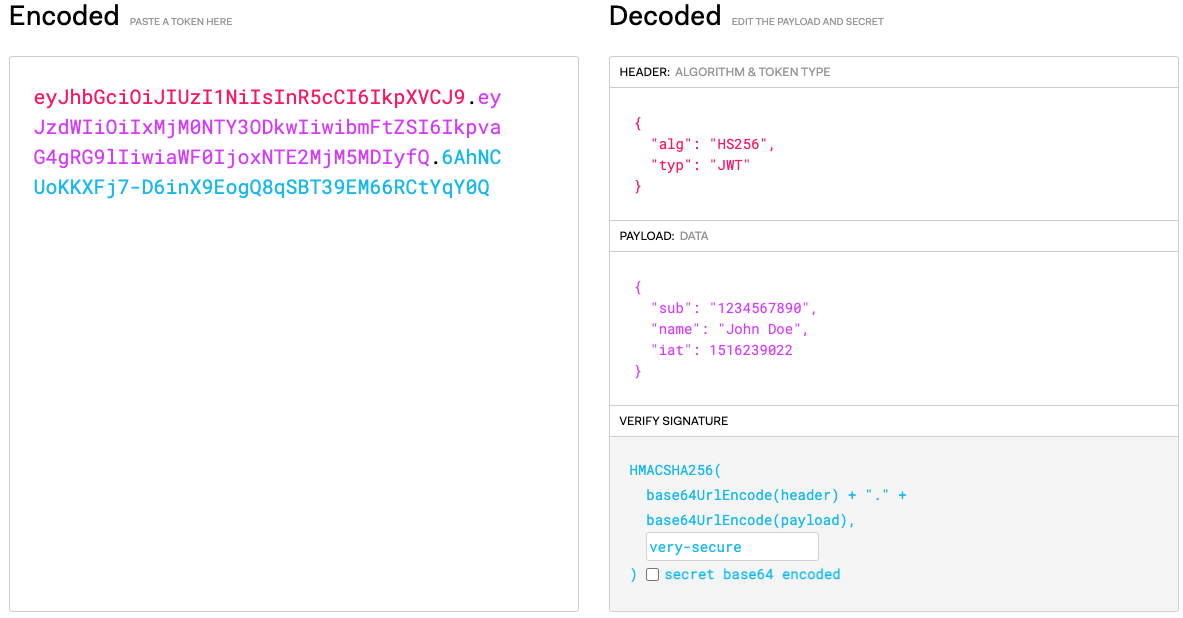
\includegraphics[width=.95\linewidth]{./images/jwt.io.png}
  \caption[{Screenshot von JWT.io}]{Screenshot von JWT.io}
  \label{fig:jwt}
\end{figure}
\subsection{Anwendung} \label{andwendung-jwt}
Bei einer erfolgreichen Anmeldung erstellt das Backend einen JWT. Dessen Inhalt ist die Id des Nutzers, die Email, ein Boolean womit das Frontend weiss, ob der User bereits ein Modell registriert hat, das Erstellungsdatum und das Verfallsdatum. Dieser wird an das Frontend zurückgegeben. Das Frontend speichert diesen im SessionStorage und sendet ihn bei jeder weiteren Anfrage mit. Somit weiss das Backend immer, wer die Anfrage erstellt hat.
\newline
Sollte zum Beispiel die Id des Nutzers im  JWT verändert werden, stimmt die Signatur nicht mehr und das Backend lehnt die Anfrage mit dem HTTP Status Code 401 ab.